%
% exemplo genérico de uso da classe iiufrgs.cls
% $Id: iiufrgs.tex,v 1.1.1.1 2005/01/18 23:54:42 avila Exp $
%
% This is an example file and is hereby explicitly put in the
% public domain.
%
\documentclass[cic,tc]{iiufrgs}
% um tipo específico de monografia pode ser informado como parâmetro opcional:
%\documentclass[tese]{iiufrgs}
% monografias em inglês devem receber o parâmetro `english':
%\documentclass[diss,english]{iiufrgs}
% a opção `openright' pode ser usada para forçar inícios de capítulos
% em páginas ímpares
% \documentclass[openright]{iiufrgs}
% para gerar uma versão somente-frente, basta utilizar a opção `oneside':
% \documentclass[oneside]{iiufrgs}
\usepackage[utf8]{inputenc}   % pacote para acentuação
\usepackage{times}              % pacote para usar fonte Adobe Times
\usepackage[alf,abnt-emphasize=bf]{abntex2cite}	% pacote para usar citações abnt
\usepackage{graphicx}          % para inserir imagens
\usepackage{booktabs}
\usepackage{float}     % para as imagens ficarem no lugar certo
%\usepackage{mathptmx}          % p/ usar fonte Adobe Times nas fórmulas
\usepackage{multirow}
\usepackage{amsmath}

\graphicspath{ {images/} }

\title{Uma análise dos dados de queimada do INPE no Brasil (preliminar)}
\translatedtitle{Using \LaTeX\ to Prepare Documents at II/UFRGS}

\author{Braz}{José Henrique da Silva}
\advisor[Prof.~Dr.]{Schnorr}{Lucas M.}

% a data deve ser a da defesa; se nao especificada, são gerados
% mes e ano correntes
%\date{maio}{2001}

% o nome do curso pode ser redefinido (ex. para TCs)
\course{Curso de Graduação em Ciência da Computação}

% o local de realização do trabalho pode ser especificado (ex. para TCs)
% com o comando \location:
\location{Porto Alegre}{RS}

% palavras-chave
% iniciar todas com letras maiúsculas
%
\keyword{Formatação eletrônica de documentos}
\keyword{\LaTeX}
\keyword{ABNT}
\keyword{UFRGS}

%
% palavras-chave na lingua estrangeira
% iniciar todas com letras maiúsculas
%
\translatedkeyword{Electronic document preparation}
\translatedkeyword{\LaTeX}
\translatedkeyword{ABNT}
\translatedkeyword{UFRGS}

%
% inicio do documento
%
\begin{document}

% folha de rosto
% às vezes é necessário redefinir algum comando logo antes de produzir
% a folha de rosto:
% \renewcommand{\coordname}{Coordenadora do Curso}
\maketitle

% dedicatoria
\clearpage
\begin{flushright}
\mbox{}\vfill
{\sffamily\itshape
``If I have seen farther than others,\\
it is because I stood on the shoulders of giants.''\\}
--- \textsc{Sir~Isaac Newton}
\end{flushright}

% agradecimentos
\chapter*{Agradecimentos}
Agradeço ao \LaTeX\ por não ter vírus de macro\ldots

% sumario
\tableofcontents

% lista de abreviaturas e siglas
% o parametro deve ser a abreviatura mais longa
% A NBR 14724:2011 estipula que a ordem das abreviações
% na lista deve ser alfabética (como no exemplo abaixo).
\begin{listofabbrv}{SPMD}
	\item[ABI] Advanced Baseline Imager
	\item[API] Application Programming Interface (Interface de Programação de Aplicação)
	\item[ATRS] Along Track Scanning Radiometer
	\item[AVHRR] Advanced Very High Resolution Radiometer
	\item[CSV] Comma Separated Values (valores separados por vírgulas)
	\item[EUMETSAT] European Organisation for the Exploitation of Meteorological Satellites
	\item[ESA] European Space Agency
    \item[GMT] Greenwich Mean Time
    \item[GOES] Geostationary Operational Environmental Satellite
    \item[INPE] Instituto Nacional de Pesquisas Espaciais
    \item[IBGE] Instituto Brasileiro de Geografia e Estatística
    \item[JAXA] Japan Aerospace Exploration Agency
    \item[URL] Uniform Resource Locator (Localizador Uniforme de Recursos)
    \item[NASA] National Aeronautics and Space Administration
    \item[NOAA] National Oceanic and Atmosphere Administration
    \item[MSG] Meteosat Second Generation
    \item[METOP] Meteorological Operational Satellite
    \item[MODIS] Moderate Resolution Imaging Spectroradiometer
    \item[TRMM] Tropical Rainfall Measuring Mission
    \item[WRS] Worldwide Reference System
    \item[VIIRS] Visible Infrared Imaging Radiometer Suite
\end{listofabbrv}

% idem para a lista de símbolos
%\begin{listofsymbols}{$\alpha\beta\pi\omega$}
%       \item[$\sum{\frac{a}{b}}$] Somatório do produtório
%       \item[$\alpha\beta\pi\omega$] Fator de inconstância do resultado
%\end{listofsymbols}

% lista de figuras
\listoffigures

% lista de tabelas
\listoftables

% resumo na língua do documento
\begin{abstract}
Este documento é um exemplo de como formatar documentos para o
Instituto de Informática da UFRGS usando as classes \LaTeX\
disponibilizadas pelo UTUG\@. Ao mesmo tempo, pode servir de consulta
para comandos mais genéricos. \emph{O texto do resumo não deve
conter mais do que 500 palavras.}
\end{abstract}

% resumo na outra língua
\begin{translatedabstract}
This document is an example on how to prepare documents at II/UFRGS
using the \LaTeX\ classes provided by the UTUG\@. At the same time, it
may serve as a guide for general-purpose commands. \emph{The text in
the abstract should not contain more than 500~words.}
\end{translatedabstract}

% aqui comeca o texto propriamente dito

%%%%%%%%%%%%%%%%%%%%%%%%%%%%%%%%%%%%%%%%%%%%%%%%%%%%%%%%%%%%%%%%%%%%%%%%%%%%%%%

\chapter{Introdução}

O fogo é uma tecnologia que está presente há milênios no território que hoje é o Brasil, desde queimadas controladas pelo povo indígena Kayapó no cerrado para plantio ou caça, até incêndios iniciados por combustão espontânea em períodos de seca no sul da Amazônia. O uso do fogo pelos indígenas era controlado, levando em conta o clima atual e a vegetação a ser queimada, e restrito apenas a um período do ano, com o intuito de reduzir pragas e ajudar nas plantações \citep{leonel_2000}. [P0. O que é uma queimada/fogo] \par

Hoje as queimadas que mais chamam atenção estão diretamente ligadas ao processo de desmatamento e manejo de áreas agrícolas para o cultivo da monocultura de soja. O fogo também é a prática mais barata e rápida para limpar áreas inteiras para a pecuária bovina. Commodites agrícolas e carne bovina movem a economia do Brasil, que é o maior exportador desses produtos, e aumentam a pressão para o desmatamento de novas áreas na Amazônia \citep{fuchs_2020}. [P1. As queimadas hoje] \par

O Brasil ocupa a quarta posição no ranking de nações que mais emitem gases de efeito estufa por habitantes, segundo dados da United Nations Environment Programme (UNEP) de 2022. De acordo com o estudo, o valor absoluto se manteve estável desde 2010, e atingiu seu pico por volta dos anos de 2003 a 2004. Assim como a Indonésia, o que melhor explica a alta posição do Brasil neste ranking são as queimadas e o desmatamento da vegetação nativa. Olhando para os municípios do país, dos dez que mais poluem, oito deles estão localizados no bioma da amazônia e não possuem atividades industriais que justificariam esse valor. [P2. queimadas e efeito estufa no Brasil] \par

\begin{figure}[H]
    \caption{Emissões de gases do efeito estufa per capta de 1990 até 2020 (tCO2e/capita).}
    \begin{center}
        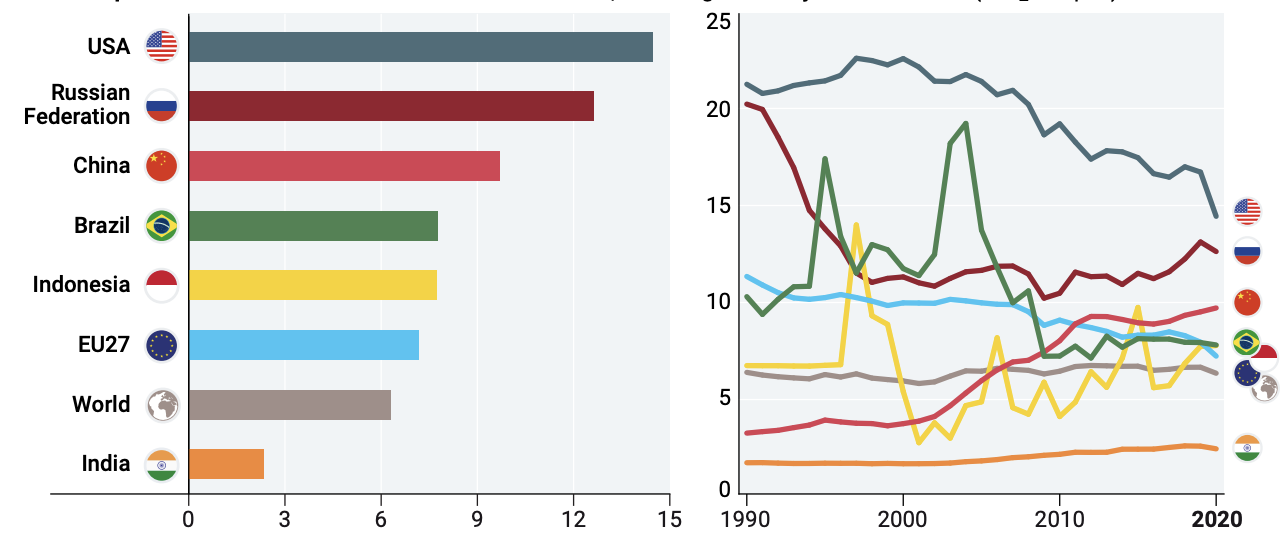
\includegraphics[width=35em]{emissoes_gee_per_capta}
    \end{center}
    \legend{Fonte: Emissions Gap Report 2022: The Closing Window}
    \label{fig:emissoes_gee_per_capta}
\end{figure}

Este trabalho se dedica a estudar e apresentar de forma concisa os dados de focos de queimadas disponibilizados pelo Instituto Nacional de Pesquisas Espaciais (INPE). O principal objetivo é tornar fácil o entendimento desses dados gerados a partir de imagens de satélites, sem a necessidade de um conhecimento prévio das técnicas de ciência de dados e sensoriamento remoto. O escopo de tempo das análises é limitado ao início de 1998, ano que iniciou a base aberta de queimadas, até o final de 2022. 

Os dados analisados neste trabalho foram obtidos a partir do DBQueimadas, Banco de Dados de Queimadas \url{www.inpe.br/queimadas/bdqueimadas}, que é um sistema desenvolvido pelo INPE e acessível de forma aberta por meio da web. Conta com mais de 300 milhões de pontos coletados desde o ano de 1998, provenientes de vários satélites \citep{setzer2019banco}. Ao disponibilizar os dados das queimadas o instituto possibilita que a sociedade retribua com pesquisas e fomenta novas abordagens ao problema das queimadas no Brasil, como é o caso deste trabalho.

... apontaram que a detecção de áreas queimadas pode se beneficiar da fusão de observações de incêndios ativos de vários sensores \citep{giglio2010assessing}.

Focos ativos apresentam maior contraste com a vegetação e por isso podem ser detectados com maior precisão \citep{GIGLIO2016}, mas devido ao intervalo entre as passagens dos satélites, detectam apenas uma fração das queimadas totais \citep{HANTSON2013, giglio2009active}. .......

tem muita variação entre os produtos de queimadas .... \citep{Boschetti2004}

\citep{Humber2019} 


Durante o decorrer do documento são apresentadas diversas figuras, a maioria de construção do próprio autor, a fim de instigar a intuição do leitor para o tópico que está sendo abordado. De início, é abordado questões mais teóricas envolvendo caracteríscas dos satélites, suas produções de imagens e como são usadas para detectar um foco ativo de queimada. Após isso, .... \par


%%%%%%%%%%%%%%%%%%%%%%%%%%%%%%%%%%%%%%%%%%%%%%%%%%%%%%%%%%%%%%%%%%%%%%%%%%%%%%%

\chapter{Conceitos básicos e trabalhos relacionados}

Neste Capítulo, serão apresentados conceitos importantes para a compreensão de todo trabalho e dos resultados obtidos com o método proposto. Primeiramente, serão formalizadas definições relacionadas às queimadas e à forma como são monitoradas no Brasil. Na próxima seção, é realizada uma sumarização dos principais satélites utilizados pelo INPE e suas características. Após isso, apresentamos uma análise dos dados para demonstrar uma visão geral das principais tendências e gráficos. Em seguida, é abordado como as imagens geradas pelos satélites são utilizadas para a detecção de focos ativos. Por fim, apresentamos alguns trabalhos relacionados com o cálculo de área queimada em contraste com o presente trabalho. \par

\section{O monitoramento das queimadas no Brasil}

Um foco de queima, também conhecido como ``Fire Pixel'', é a detecção de fogo na vegetação por uma imagem de satélite. A área de abrangência dessa detecção é do tamanho de um pixel da imagem, por isso está relacionada diretamente com a resolução do sensor do satélite. Por exemplo, se um sensor tem resolução de aproximadamente 1km, a área coberta pelo pixel equivale a 1km no nadir (no equador) \cite{PerguntasFrequentesINPE}. A resolução do sensor, na verdade, representa uma estimativa do tamanho dos pixels, pois eles podem sofrer distorções relacionadas a inclinação e distância do satélite em relação ao ponto medido. 

É importante destacar que o foco de queima por si só não representa de forma precisa o que está acontecendo na região, mas é um indicador valioso da intensidade e extensão do fogo. Poucos focos ou uma área queimada pequena não necessariamente refletem a intensidade da degradação da vegetação e o impacto ambiental. Áreas de floresta densa, mesmo que pequenas, podem ser gravemente afetadas, resultando em perdas significativas de fauna e flora, incluindo espécies exóticas e em risco de extinção.

Um incêndio, diferente de um foco de queima, pode durar dias e queimar uma grande extensão de terra, o que provavelmente resulta na detecção de vários focos de queima. O número de focos de queima está diretamente relacionado à extensão total queimada e pode ser utilizado para comparações e análises \citep{giglio2010assessing}. A área queimada, por outro lado, representa o resultado deixado pelo incêndio, que também pode ser estimada a partir de imagens de satélites. Existem vários métodos para detectar focos ativos e calcular a área queimada a partir dos dados brutos de satélites, alguns deles são abordados no decorrer do documento. 

Para monitorar e proteguer o meio ambiente do Brasil das queimadas, o INPE desenvolve o programa de Monitoramento de Queimadas e Incêndios Florestais (\url{https://queimadas.dgi.inpe.br/queimadas/portal}). O programa é um conjunto de ferramentas abertas, muitas delas acessíveis via Web, desenvolvidas pelo time de tecnologia do INPE que possibilitam obter e visualizar dados sobre os focos de queimadas, risco de fogo, área queimada, focos em áreas de preservação e propriedades rurais, entre outras.

O programa também conta com o Banco de Dados de Queimadas (DBQueimadas), um site capaz de gerar mapas, tabelas, gráficos e exportar os dados sobre as queimadas no Brasil aplicando diferentes filtros \citep{setzer2019banco}. O DBQueimadas é um excelente caso de como os dados abertos podem ajudar a sociedade, pois qualquer pessoa pode ter acesso aos dados e desenvolver trabalhos científicos, fomentando a ciência e melhorando o monitoramento. É a partir do DBQueimadas que este trabalho obteve boa parte dos dados necessários para o desenvolvimento.

Além do DBQueimadas, o INPE também disponibiliza para visualização e download, por meio da Divisão de Geração de Imagens (DGI) \url{www.dgi.inpe.br/catalogo/}, algumas imagens inteiras geradas pelos satélites que o próprio DGI captura e processa. Para obter essas imagens brutas são necessárias antenas especiais que ficam em centros de recepção de dados. Com esse propósito, a DGI possui duas Estações de Recepção e Gravação (ERG) - a primeira em Cachoeira Paulista (SP) e uma mais recente em Cuiabá (MT). Na estação de SP, é feito o processamento de mais de 200 imagens de diversos satélites todos os dias, extraindo os dados de focos ativos de queimadas que alimentam o DBQueimadas \citep{SiteDGI}. \par

É em posse dessas imagens que o INPE aplica algoritmos de detecção de focos de queima, abordado na Seção \ref{sec:deteccao_focos_section}. No caso da detecção ser positiva, a posição exata (latitude e longitude) e a hora que a imagem foi gerada são adicionadas aos dados como uma nova linha e disponibilizados pelo DBQueimadas. O INPE ainda coloca junto com as coordenadas da detecção mais alguns dados como risco de fogo, poder do fogo, precipitação e dados referentes a região do foco. A lista completa da estrutura dos dados pode ser vista na Tabela \ref{table:inpeColumns}, nela a coluna Atributo indica o nome de cada coluna nos dados, seguido do tipo e uma breve descrição \cite{PerguntasFrequentesINPE}. \par

\begin{table}[htbp]
\centering
\caption{Significado de cada coluna dos dados de queimada do INPE.}
\begin{tabular}{@{}llp{9cm}@{}}
 \toprule
 \textbf{Atributo} & \textbf{Tipo} & \textbf{Descrição} \\
 \midrule
 \texttt{Id} & \texttt{string} & Identificador único registrado no banco \\
 \texttt{Latitude} & \texttt{double} & Graus decimais da latitude do centro 
                     do pixel de fogo ativo (valores de 90.0000 até -90.0000) \\ 
 \texttt{Longitude} & \texttt{double} & Graus decimais da longitude do centro 
                     do pixel de fogo ativo (valores de 180.0000 até -180.0000) \\  
 \texttt{DataHora} & \texttt{string} & Data a hora da passagem do satélite no fuso 
                     horário de Greenwich (GMT) \\   
 \texttt{Municipio} & \texttt{string} & Nome do município, de acordo com os dados 
                     do IBGE 2000 \\
 \texttt{Estado} & \texttt{string} & Nome do estado \\
 \texttt{Pais} & \texttt{string} & Nome do país \\  
 \texttt{Bioma} & \texttt{string} & Nome do bioma brasileiro, de acordo com 
                     dados do IBGE 2004 (para outros países o campo fica vazio) \\
 \texttt{Precipitação} & \texttt{double} & Valor a precipitação do dia até 
                     o horário da medida (-999 para valores inválidos) \\
 \texttt{DiasSCh} & \texttt{integer} & Dias sem chuva até a data da medida 
                     (-999 para valores inválidos) \\
 \texttt{RiscoFog} & \texttt{double} & Valor do risco de fogo previsto naquele dia 
                     (-999 para valores inválidos) \\
 \texttt{FRP} & \texttt{double} & Fire Radiative Power, MW (megawatts) \\
 \bottomrule
\end{tabular}
\legend{Fonte: \citet{PerguntasFrequentesINPE}}
\label{table:inpeColumns}
\end{table}

\section{Os Satélites e Sensores}

O INPE processa atualmente dados de diversos satélites, cada um com características distintas. Esses satélites abrangem uma ampla gama de órbitas e altitudes, desde satélites geoestacionários, como o GOES-12, localizado a 29.400 km de distância da superfície \citep{GOES12Algo}, até satélites em órbitas polares, que ficam entre 700 e 900 km de altura. Cada um deles é equipado com diferentes sensores que são utilizados para diversos propósitos, como observação da vegetação terrestre, nuvens, oceanos e monitoramento atmosférico. \par

Cada satélite pode estar equipado com um sensor imageador que captura imagens com características distintas. Esses sensores são capazes de captar não apenas a luz visível, no comprimento de onda de 400 nm a 700 nm, mas também o infravermelho, de 780 nm a 1 mm. As medições realizadas pelos sensores são divididas em canais, que diferem em termos de resolução espacial - a escala geográfica representada por cada pixel da imagem - e resolução espectral, ou seja, o intervalo de comprimento de onda abrangido. \par

Os satélites também podem ser classificados de acordo com o tipo de órbita, que pode ser polar ou geoestacionária. Os satélites polares percorrem toda a terra, com uma altitude baixa e alta velocidade, passando várias vezes pelos polos norte e sul em um único dia. Já os satélites geoestacionários ajustam sua orbita para sempre parecerem estacionários em relação a um ponto fixo na Terra. Esses satélites ficam em altitudes mais altas devido à sua velocidade mais baixa, que é igual à rotação da Terra. A Figura \ref{fig:orbita2022-08-10}, gerada a partir de dados do site Celestrak (\url{https://celestrak.org/}), mostra a passagem de alguns satélites polares no Brasil no dia 10 de agosto de 2022. Também é possível ver o satélite geoestacioário GOES-16, localizado ao norte do perú, representado com um ponto no gráfico. \par

\begin{figure}[H]
    \caption{Órbita dos satélites no dia 10 de agosto de 2022.}
    \begin{center}
        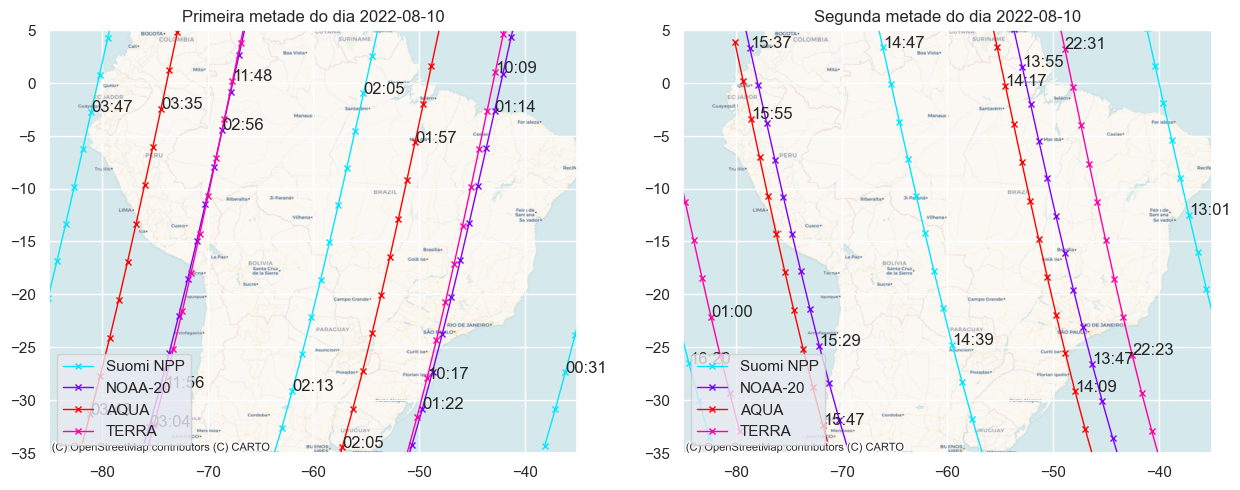
\includegraphics[width=35em]{orbita2022-08-10}
    \end{center}
    \legend{Fonte: O Autor}
    \label{fig:orbita2022-08-10}
\end{figure}

A Tabela \ref{table:satelites} contém um resumo dos satélites utilizados pelo INPE desde o início da série histórica até o final de 2022 \cite{EmbrapaSatelites}. Na Tabela, são apresentados o nome do satélite, o nome do sensor imageador, a resolução espacial do sensor, o tipo de órbita do satélite, o ano em que o satélite entrou em operação e, por último, os dois horários aproximados da passagem de um satélite polar no território do Brasil. Os horários exatos dessa passagem variam de acordo com a excentricidade da órbita do satélite o que reflete no chamado ``Periodo de revisita'', que indica quantos dias o satélite leva para repetir a mesma tragetória.

\begin{table}[htbp]
\centering
\caption{Características dos satélites usados pelo INPE.}
\begin{tabular}{ @{}llllcl@{} }
  \toprule
  \textbf{Nome}    & \textbf{Sensor} & \textbf{Res. esp.} & \textbf{Órbita} & \textbf{Lançado} & \textbf{Passagem no Brasil} \\
  \midrule
  NOAA-12 & AVHRR    & 1100m       & Polar   & 1991 & 2h / 15h \\
  ERS-1   & ATSR-1   & 1000m       & Polar   & 1991 & Variadas \\
  NOAA-14 & AVHRR    & 1100m       & Polar   & 1994 & 21h \\
  ERS-2   & ATSR-2   & 1000m       & Polar   & 1995 & Variadas \\
  TRMM    & VIRS     & 2000m       & Polar   & 1997 & Variadas \\
  NOAA-15 & AVHRR-3  & 1100m       & Polar   & 1998 & 5h / 17h \\
  TERRA   & MODIS    & 1000m       & Polar   & 1999 & 11h / 23h \\
  NOAA-16 & AVHRR-3  & 1100m       & Polar   & 2000 & Variadas \\
  AQUA    & MODIS    & 1000m       & Polar   & 2002 & 2h / 14h \\
  NOAA-17 & AVHRR-3  & 1100m       & Polar   & 2002 & 21h \\
  NOAA-18 & AVHRR-3  & 1100m       & Polar   & 2005 & Variadas \\
  NOAA-19 & AVHRR-3  & 1100m       & Polar   & 2009 & 2h / 14h \\
  Suomi NPP & VIIRS  & 500m        & Polar   & 2011 & 2h / 14h \\
  METOP-B & AVHRR-3  & 1100m       & Polar   & 2012 & 21h \\
  NOAA-20 & VIIRS    & 500m        & Polar   & 2017 & 2h / 14h \\
  METOP-C & AVHRR-3  & 1100m       & Polar   & 2018 & 21h \\
  GOES-08 & GOES I-M & 4000m       & Geoest. & 1994 & Não se aplica \\
  GOES-10 & GOES I-M & 4000m       & Geoest. & 1997 & Não se aplica \\
  GOES-12 & GOES I-M & 4000m       & Geoest. & 2001 & Não se aplica \\
  MSG-02  & SEVIRI   & 3000m       & Geoest. & 2005 & Não se aplica \\
  GOES-13 & GOES I-M & 4000m       & Geoest. & 2006 & Não se aplica \\
  MSG-03  & SEVIRI   & 3000m       & Geoest. & 2012 & Não se aplica \\
  GOES-16 & ABI      & 2000m       & Geoest. & 2016 & Não se aplica \\
  \bottomrule
\end{tabular}
\legend{Fonte: O Autor com base em \citet{EmbrapaSatelites}}
\label{table:satelites}
\end{table}

Atualmente, os satélites que estão em pleno funcionamento são: NOAA-20, NOAA-19, NOAA-18, GOES-16, Suomi NPP, AQUA, TERRA, MSG-03, METOP-B e METOP-C. Os demais satélites, como NOAA-17, NOAA-16, NOAA-15, TRMM, NOAA-14, NOAA-12, GOES-13, MSG-02, GOES-12, GOES-10 e GOES-08, deixaram de operar em diferentes momentos devido a problemas técnicos ou ao fim de sua vida útil.

Os satélites TERRA e AQUA, ambos com o sensor Moderate Resolution Imaging Spectroradiometer (MODIS), foram lançados em 1999 e 2002 respectivamente. São americanos e foram desenvolvidos em parceria com o Japão, Canada e Brasil. O sensor MODIS possui 36 canais e resolução espectral que varia de 250m a 1km em diferentes espectros do infravermelo e luz visível. É especialmente capaz de detectar mudanças no uso e cobertura da terra bem como queimadas e atividades vulcânicas.

Os satélites da série National Oceanic and Atmospheric Administration (NOAA) são operados pela agência americana de mesmo nome. Embora tenha havido vários satélites NOAA ao longo do tempo, atualmente estão em operação o NOAA-20, NOAA-19 e NOAA-18. Esses satélites desempenham um papel fundamental no fornecimento de dados para a previsão do tempo e o monitoramento da vegetação. 

Além dos satélites NOAA, em 2011, a NOAA em parceria com a National Aeronautics and Space Administration (NASA) lançou o satélite Suomi NPP (Suomi National Polar-orbiting Partnership). O Suomi NPP tem como objetivo principal obter observações ambientais e meteorológicas avançadas da Terra. É equipado com o sensor Visible Infrared Imaging Radiometer Suite (VIIRS), que também está presente no NOAA-20. Esses dois satélites, Suomi NPP e NOAA-20, são os satélites com mais alta resolução espacial entre todos os processados pelo INPE, equivalente a 250m.

O conjunto de satélites Geostationary Operational Environmental Satellite (GOES) é operado pela NASA e controlado também pelo NOAA. As primeiras versões desses satélites geoestacionários foram equipadas com o sensor GOES I-M (Imager Radiometer e Vertical Sounder) de resolução espacial equivalente a 4km. A partir do GOES-16 o sensor foi substituído pelo Advanced Baseline Imager (ABI), capaz de produzir imagens com resolução 4 vezes melhores. Esse conjunto de satélites foi e ainda é muito usado nas previsões metereológicas nos países do continente americano.

O INPE processa as imagens dos satélites da série Meteorological Operational Satellite (METOP), incluindo o METOP-B e o METOP-C, bem como os satélites da série Meteosat Second Generation (MSG), como o MSG-02 (Meteosat-9) e o MSG-03 (Meteosat-10). Ambas missões projetadas em parceria com a European Space Agency (ESA) e a European Organisation for the Exploitation of Meteorological Satellites (EUMETSAT). Esses satélites têm como objetivo a previsão do tempo, o monitoramento climático e o acompanhamento de desastres naturais. O METOP-C é o último satélite planejado para a série METOP, completando assim o conjunto de satélites METOP-A, METOP-B e METOP-C.

O instituto também processou dados dos satélites ERS-1 e ERS-2, equipados com o sensor  Along Track Scanning Radiometer (ATRS) da ESA \cite{EmbrapaSatelites}. Esses satélites, de órbita polar, são especializados em medir com precisão a temperatura da terra e dos oceanos. Os dados coletados por esses satélites são utilizados por cientistas para detectar mudanças climáticas e vegetação, incluindo eventos como queimadas, em todo o planeta. O ATRS possui duas versões, sendo que o primeiro (ATSR-1) possui 4 canais e o segundo (ATSR-2) foi aprimorado com um canal adicional para capturar a luz visível, possibilitando o monitoramento da vegetação. 

Também estão presentes nos dados, em menor escala, os focos de queimadas obtidos pelo satélite Tropical Rainfall Measuring Mission (TRMM). O TRMM foi uma missão conjunta entre a NASA e a Japan Aerospace Exploration Agency (JAXA), que teve início em 1997 e oficialmente encerrou em 2015. O principal objetivo dessa missão foi estudar a distribuição de chuvas e tempestades, bem como suas influências no clima global. \par

\subsection*{O satélite de referência}

Para estabelecer uma série temporal consistente e permitir a análise de tendências ao longo de vários anos dos focos de queimadas detectados em diferentes regiões, o INPE definiu um satélite de referência. Esse satélite de referência é escolhido com base em critérios específicos. É importante que sua órbita cubra satisfatoriamente a área do país, sem distorcer os dados de forma significativa. Além disso, é desejável que os sensores do satélite tenham resoluções adequadas, ou seja, não muito baixas, para garantir uma análise precisa dos focos de queimadas. \citep{PerguntasFrequentesINPE}

No período de 01 de junho de 1998 a 03 de julho de 2002, o satélite de referência utilizado foi o NOAA-12, com passagem no final da tarde. Após esse período, passou-se a utilizar o satélite AQUA, com passagem à tarde (identificado nos dados como AQUA\_M-T). O AQUA tem operado além da data prevista de encerramento e provavelmente deve ser descontinuado em breve. Quando isso ocorrer, a previsão é que o satélite Suomi NPP deve ser o novo satélite de referência \citep{PerguntasFrequentesINPE}. Sempre que há uma mudança de satélite de referência, a série histórica de quantidade de focos de queimada precisa ser ajustada devido a diferença entre os satélites.

\subsection*{Satélites de média resolução}

São considerados satélites de média resolução aqueles que possuem um sensor capaz de poduzir imagens em que um pixel equivale de 10 a 60 metros \citep{EmbrapaSatelites}. A principal missão que emprega esses satélites é a Landsat que lançou 9 satélites e teve início em 1972. Atualmente, apenas os satélites Landsat-8 e Landsat-9 estão ativos. Esses satélites tem período de revisita de 16 dias, ou seja, a cada 16 dias produzem dados da mesma região. 

A missão Lansat estabeleceu um sistema de órbita-ponto que divide o planeta em vários quadrantes, chama do Worldwide Reference System (WRS). A partir do Landsat-4 o WRS ganhou uma versão 2 (WRS-2), para se adequar ao fato de que os satélites passaram de 18 para 16 dias de tempo de revisita. O Brasil é coberto por 390 quadrantes, como na Figura \ref{fig:orbitas_ponto_landsat}, sendo marcados com o número da órbita e sua linha correspondente, chamado no inglês de \textit{path/row}.

\begin{figure}[H]
    \caption{Orbitas-ponto Landsat que cobrem o território brasileiro com base no WRS-2.}
    \begin{center}
        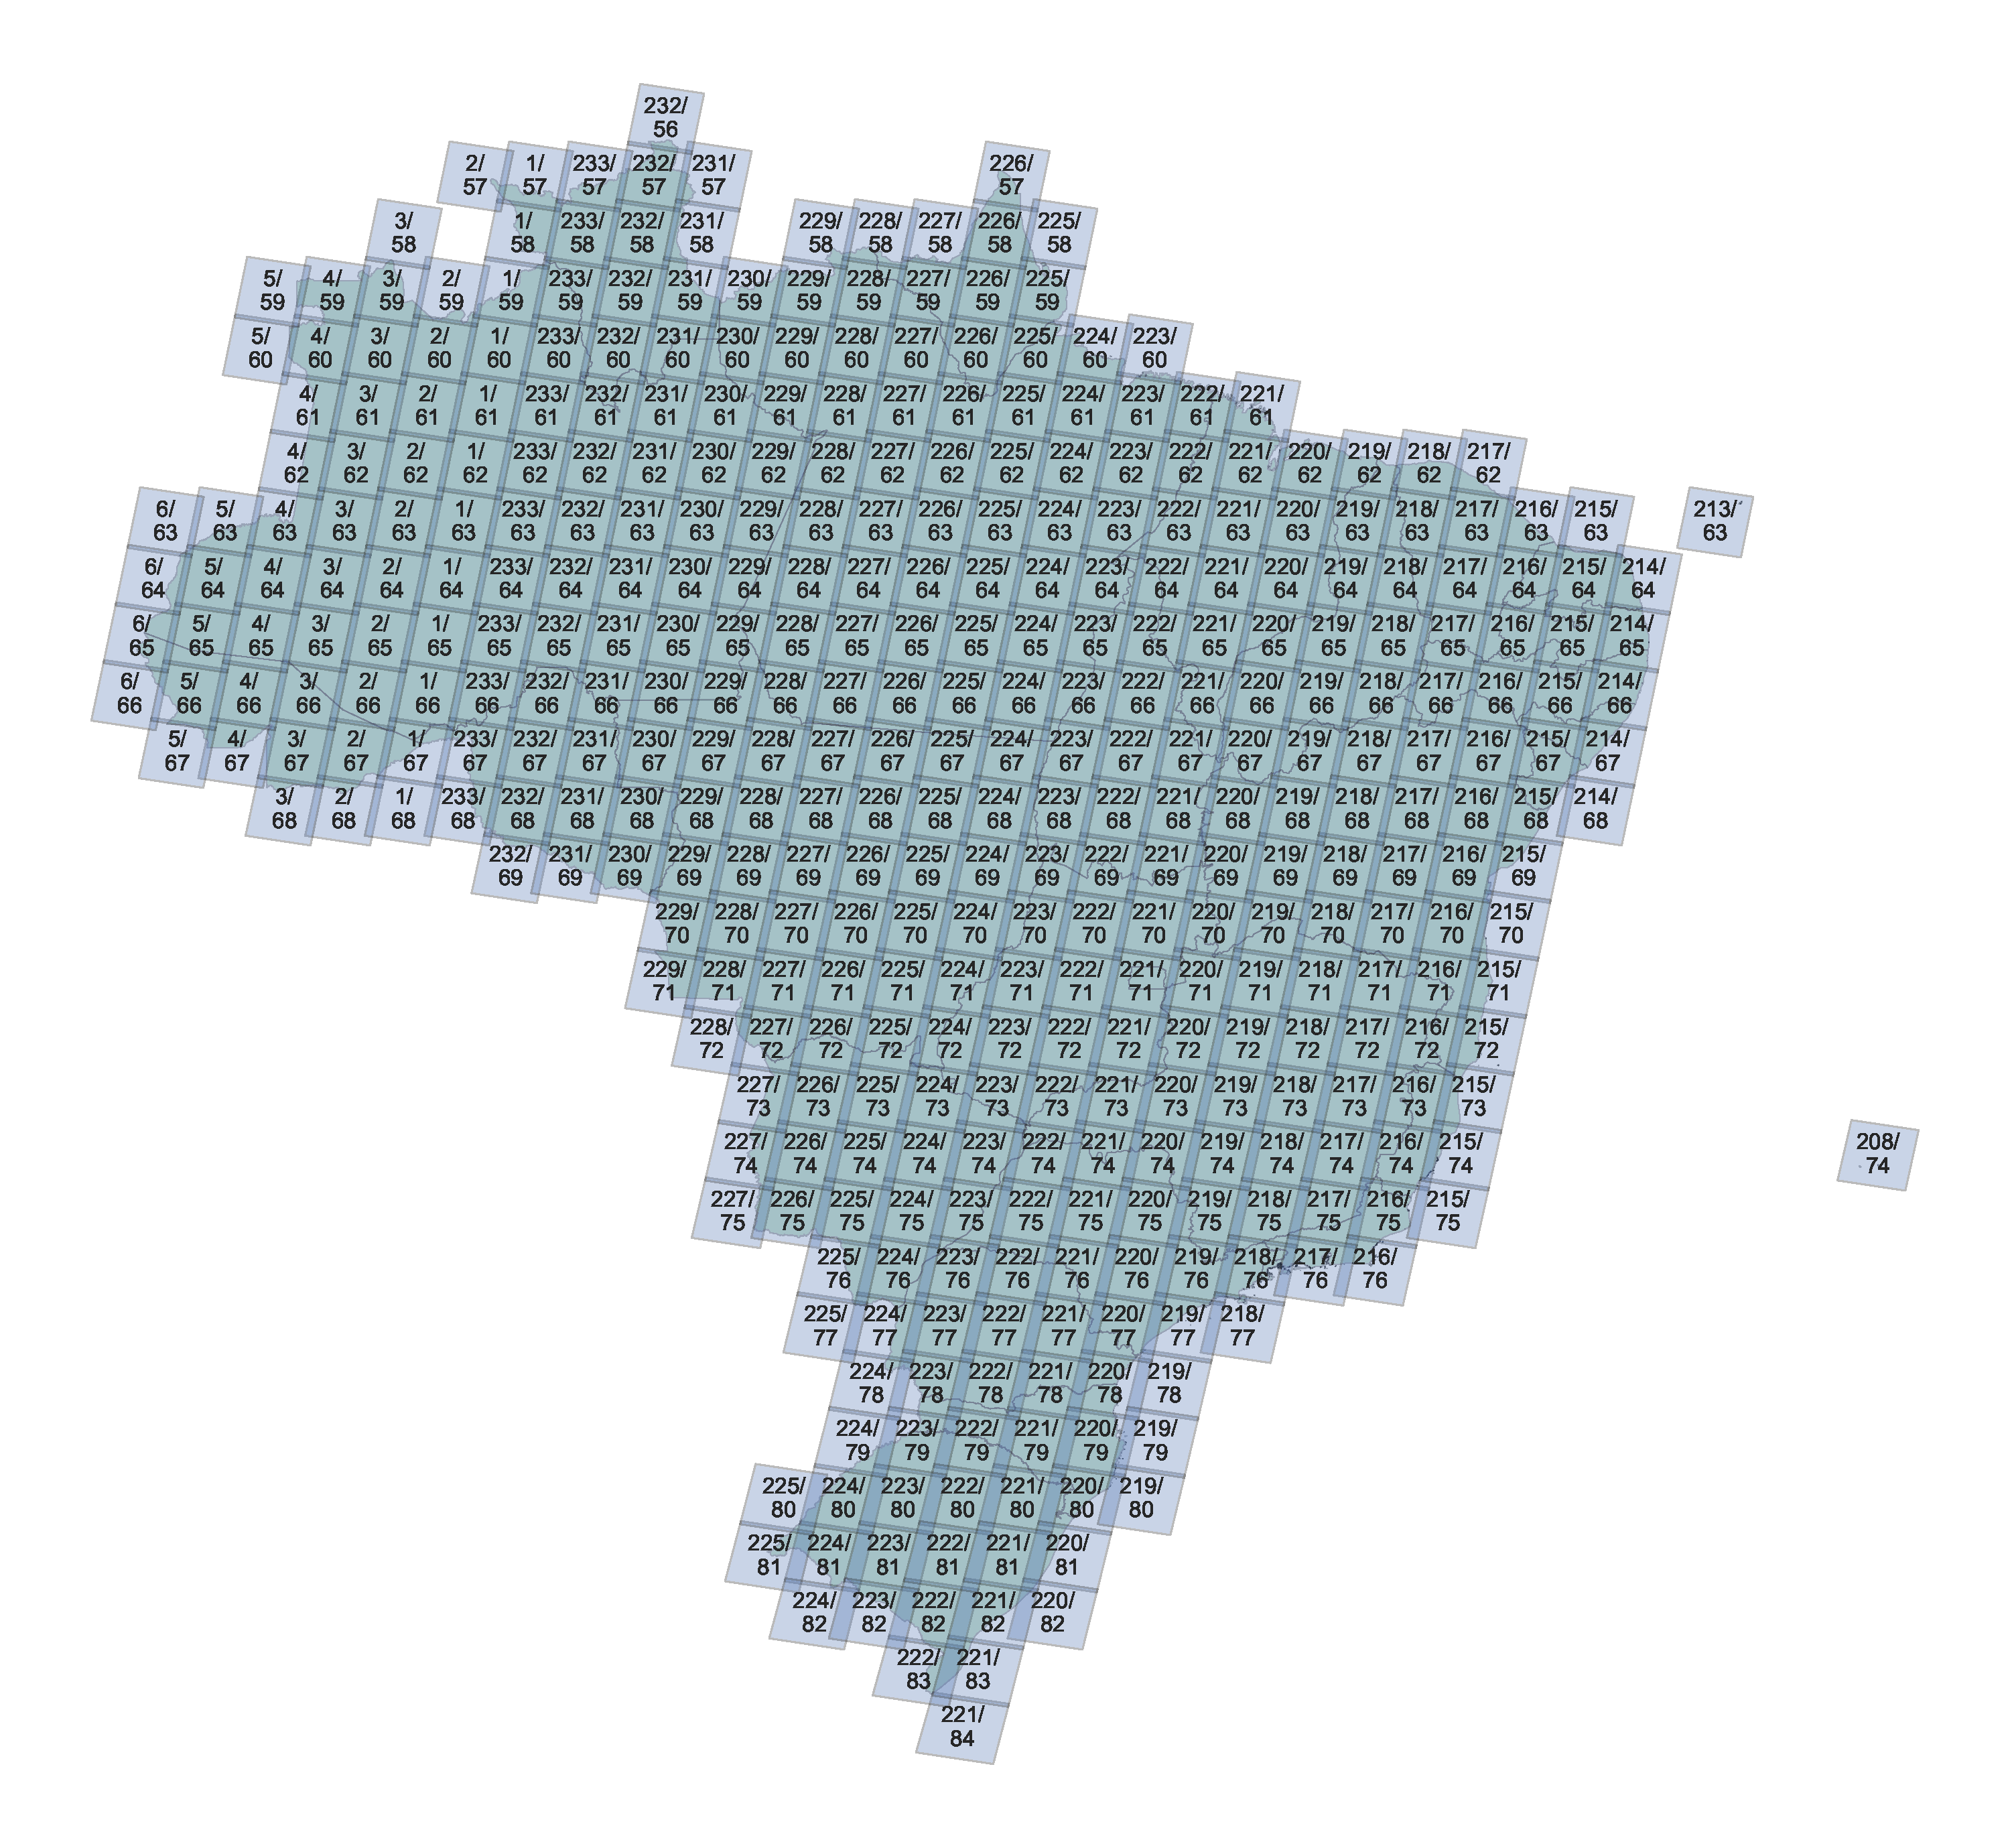
\includegraphics[width=30em]{orbitas_ponto_landsat}
    \end{center}
    \legend{Fonte: O Autor}
    \label{fig:orbitas_ponto_landsat}
\end{figure}

\section{Uma visão geral dos dados}
\label{sec:visao_geral}

Nesta seção, é realizada uma análise inicial dos dados disponíveis sobre focos de queimada, com o objetivo de extrair algumas informações relevantes. É importante, no entanto, ter cuidado na escolha dos satélites a serem utilizados na análise. Para algumas análises, caso sejam usados todos os satélites disponíveis, pode ocorrer a contagem de um mesmo foco várias vezes para diferentes satélites. Ou ainda, a contagem do mesmo foco em passagens diurnas e noturnas de um mesmo satélite polar. Para solucionar esse problema, em casos em que a quantidade absoluta de focos importa, será utilizado o satélite AQUA com passagem à tarde (AQUA\_M-T), que é o satélite de referência do INPE atualmente. Dessa forma, é possível evitar a contagem duplicada de focos de queimada e garantir a precisão das informações analisadas. 

A análise começa, na Figura \ref{fig:medicoes_nos_anos}, com uma visão preliminar sobre as características dos focos detectados durante toda a série história, para todos os satélites. Aqui é importante destacar que vários focos podem representar uma única queimada, como mencionado anteriormente, e também não há relação necessariamente direta com a área queimada. Nota-se que a série começa basicamente com os dados do satélite NOAA-12, que era o satélite de referência até 2002, e teve dados até 2007, ano que foi desativado. TERRA e AQUA foram os únicos satélites presentes no início e que até hoje tem relevância nos dados. A partir de 2012, com a entrada do satélite Suomi NPP, os dados mais que duplicaram devido a capacidade do sensor VIIRS a bordo deste satélite e depois, em 2019, junto ao satélite NOAA-20 também. A partir de 2017 o satélite GOES-16 entra em ação e, mesmo sendo geoestacionário (com menor capacidade de datecção dos focos), passou a ter relevância.


\begin{figure}[H]
    \caption{Detecções por satélite, sensor, bioma e região durante toda a série histórica}
    \begin{center}
        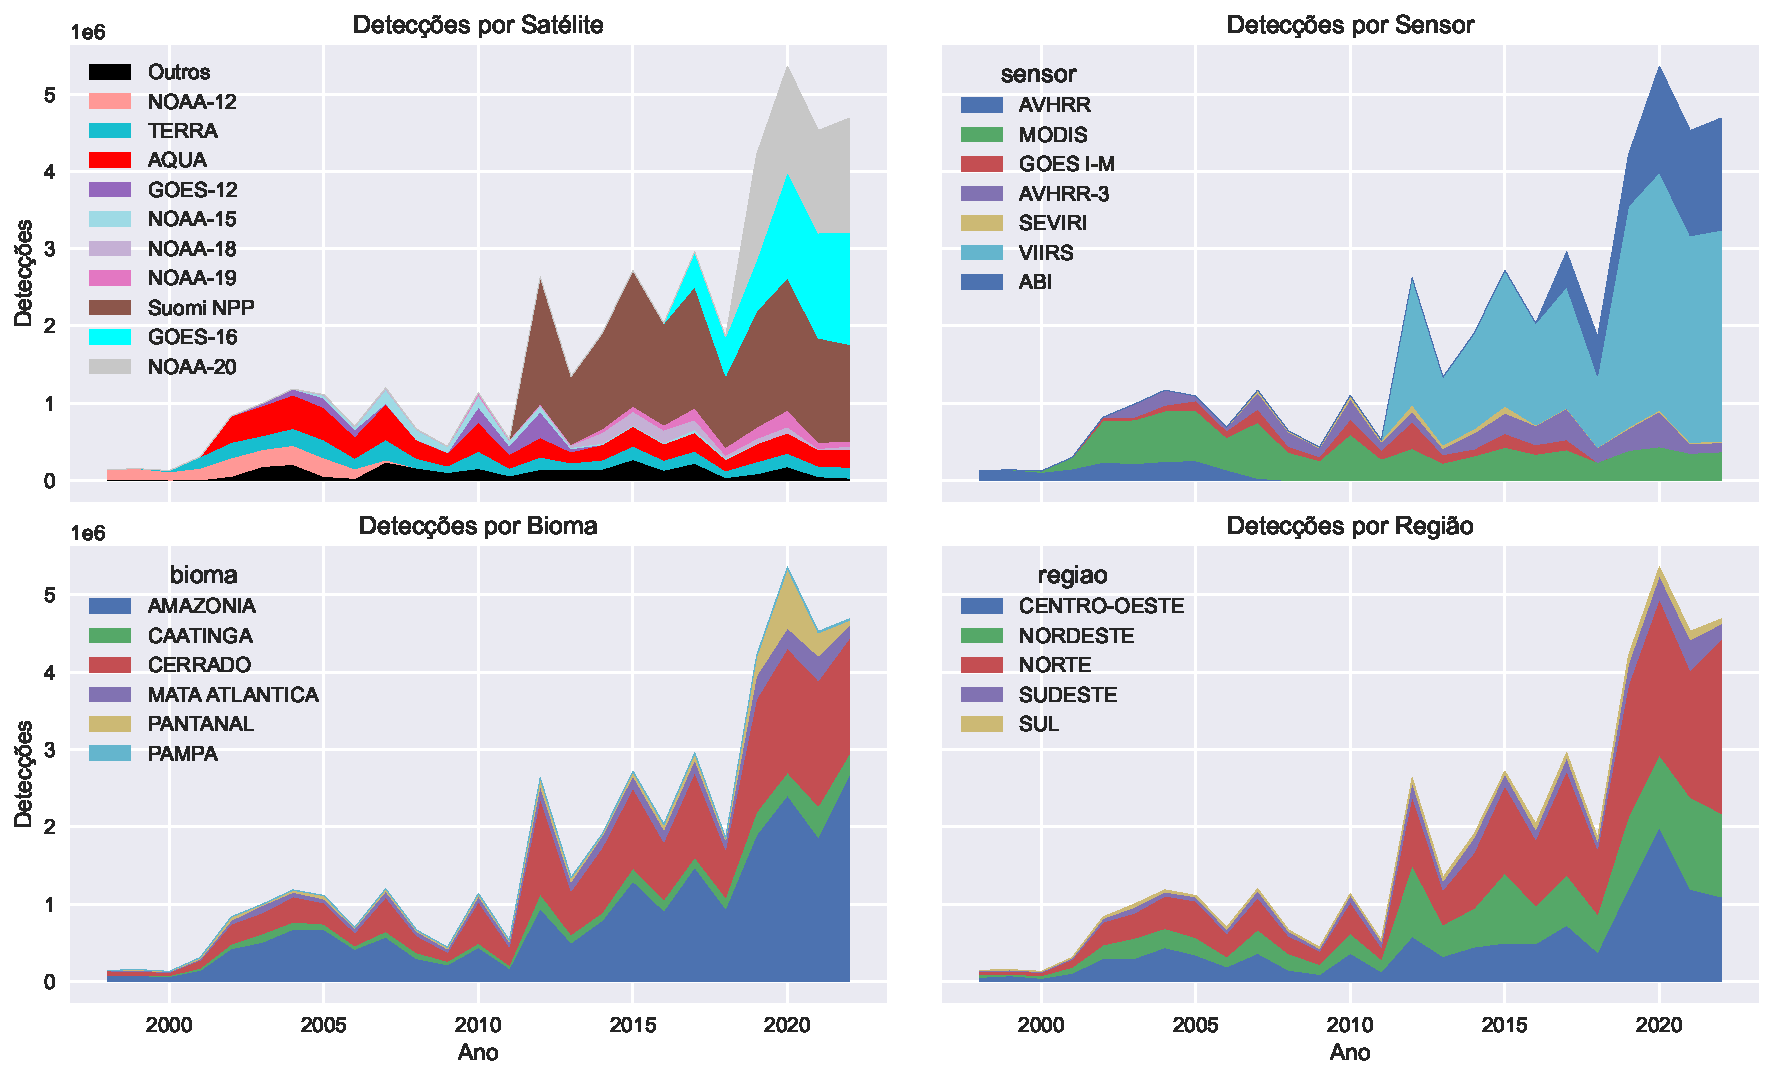
\includegraphics[width=35em]{medicoes_nos_anos}
    \end{center}
    \legend{Fonte: O Autor}
    \label{fig:medicoes_nos_anos}
\end{figure}

Quanto as detecções por bioma, nota-se que no decorrer dos anos a proporção entre os focos em cada bioma se manteve basicamente constante, com excessão do período de 2019 a 2022. Nesse período, o bioma Pantanal quebrou a tendência de ter poucos focos detectados, apresentando um aumento de 600\% e justificado por um período de seca prolongado \cite{pantanal2021dinamica}. Nesse mesmo período, também notou-se um aumento nas detecções, ainda que bem menor, no bioma da Mata Atlântica.

Saber em quais momentos os satélites passam também é importante para a análise. Os satélites polares passam duas vezes por dia no Brasil, variando o local exato da passagem de acordo com as características de sua órbita. Pela Figura \ref{fig:tempo_medidas_satelites} é possível observar esse comportamento também nos dados. As quatro primeiras linhas, que representam dados gerados por satélites polares, apresentam dois picos durante um período de 24 horas. Já para o caso dos satélites geoestacionários (GOES-16) não se observou o mesmo padrão, apresentando mais dados entre o período da tarde e início da noite, provavelmente por ser um intervalo de tempo mais quente e seco, mais propício para o fogo \citep{nepstad2007mortality}.

\begin{figure}[H]
    \caption{Amostragem por tempo de cada satélite.}
    \begin{center}
        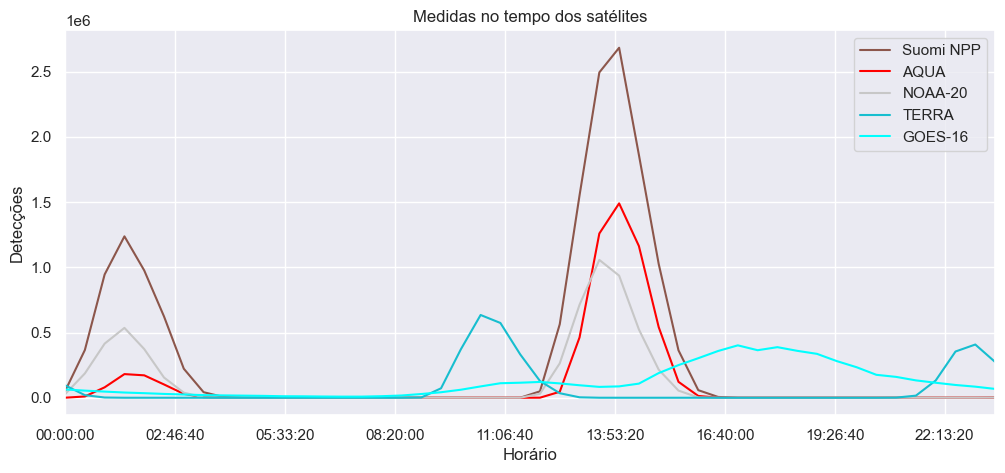
\includegraphics[width=35em]{tempo_medidas_satelites}
    \end{center}
    \legend{Fonte: O Autor}
    \label{fig:tempo_medidas_satelites}
\end{figure}

Ao realizar uma análise quantitativa dos focos de queimadas, considerando apenas o satélite de referência, é possível identificar uma sazonalidade clara na Figura \ref{fig:quantitativo_geral}. Os períodos do ano com maior número de detecções estão concentrados entre julho e setembro, com um pico máximo em 2007. Por outro lado, entre dezembro e março, as detecções diminuem significativamente, representando menos de 10\% do total de focos no ano.

\begin{figure}[H]
    \caption{Somatório dos focos do satélite de referência agrupado por mês}
    \begin{center}
        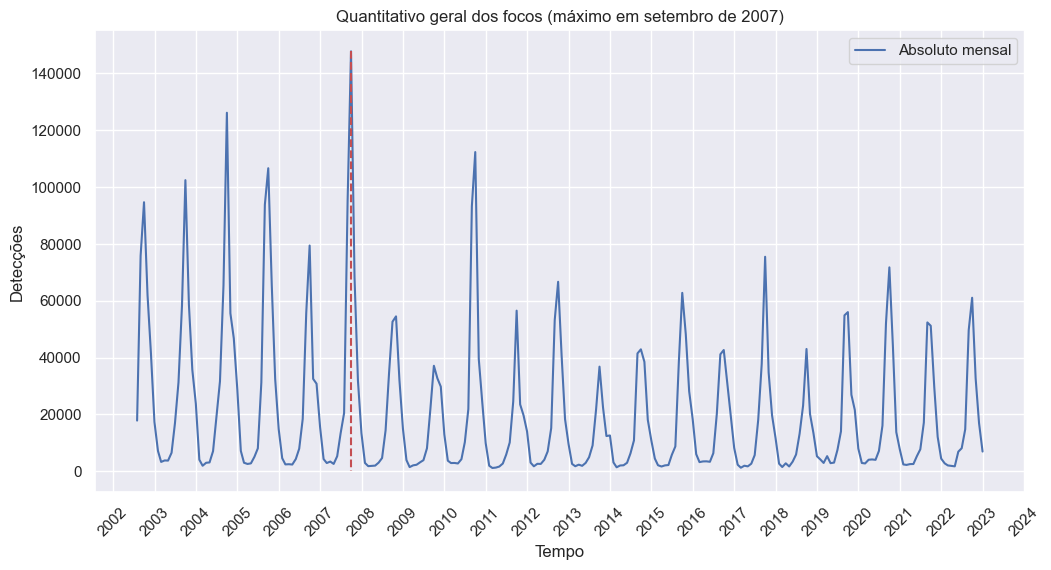
\includegraphics[width=35em]{quantitativo_geral}
    \end{center}
    \legend{Fonte: O Autor}
    \label{fig:quantitativo_geral}
\end{figure}

Esse padrão sazonal foi explicado em um estudo realizado por \citet{martins2020dinamica}. O trabalho analisou os dados de focos de queimada do satélite AQUA, obtidos pelo INPE, para o período de 2003 a 2018. Os resultados indicaram que a precipitação exerce uma influência direta na quantidade e localização dos focos no território nacional. Durante o período chuvoso, de dezembro a março, o Brasil é afetado pela Zona de Convergência Intertropical e pela Zona de Convergência do Atlântico Sul. Quando esses fenômenos estão menos intensos, a região nordeste entra em um período de seca, e à medida que a seca se intensifica, as queimadas se tornam mais frequentes e intensas.

No geral, observa-se uma tendência de queda nos focos de queimada. Tanto os períodos de baixa quanto os períodos de alta apresentam uma diminuição nas ocorrências. Essa tendência é fortemente influenciada pelos anos de 2009, 2011 e 2013, que registraram o menor número de focos, bem como pelos anos anteriores, de 2003 a 2005 e 2007, com ocorrências mais elevadas. É importante destacar que nos últimos anos, a média anual dentro de cada ano rompeu essa tendência, o que pode ser um sinal de alerta do aumento das queimadas.

\begin{figure}
    \caption{Relação de focos por área geográfica do país por município (superior esquerdo); por estado (superior direito); por região (inferior equerdo); e por bioma (inferior direito)}
    \begin{center}
        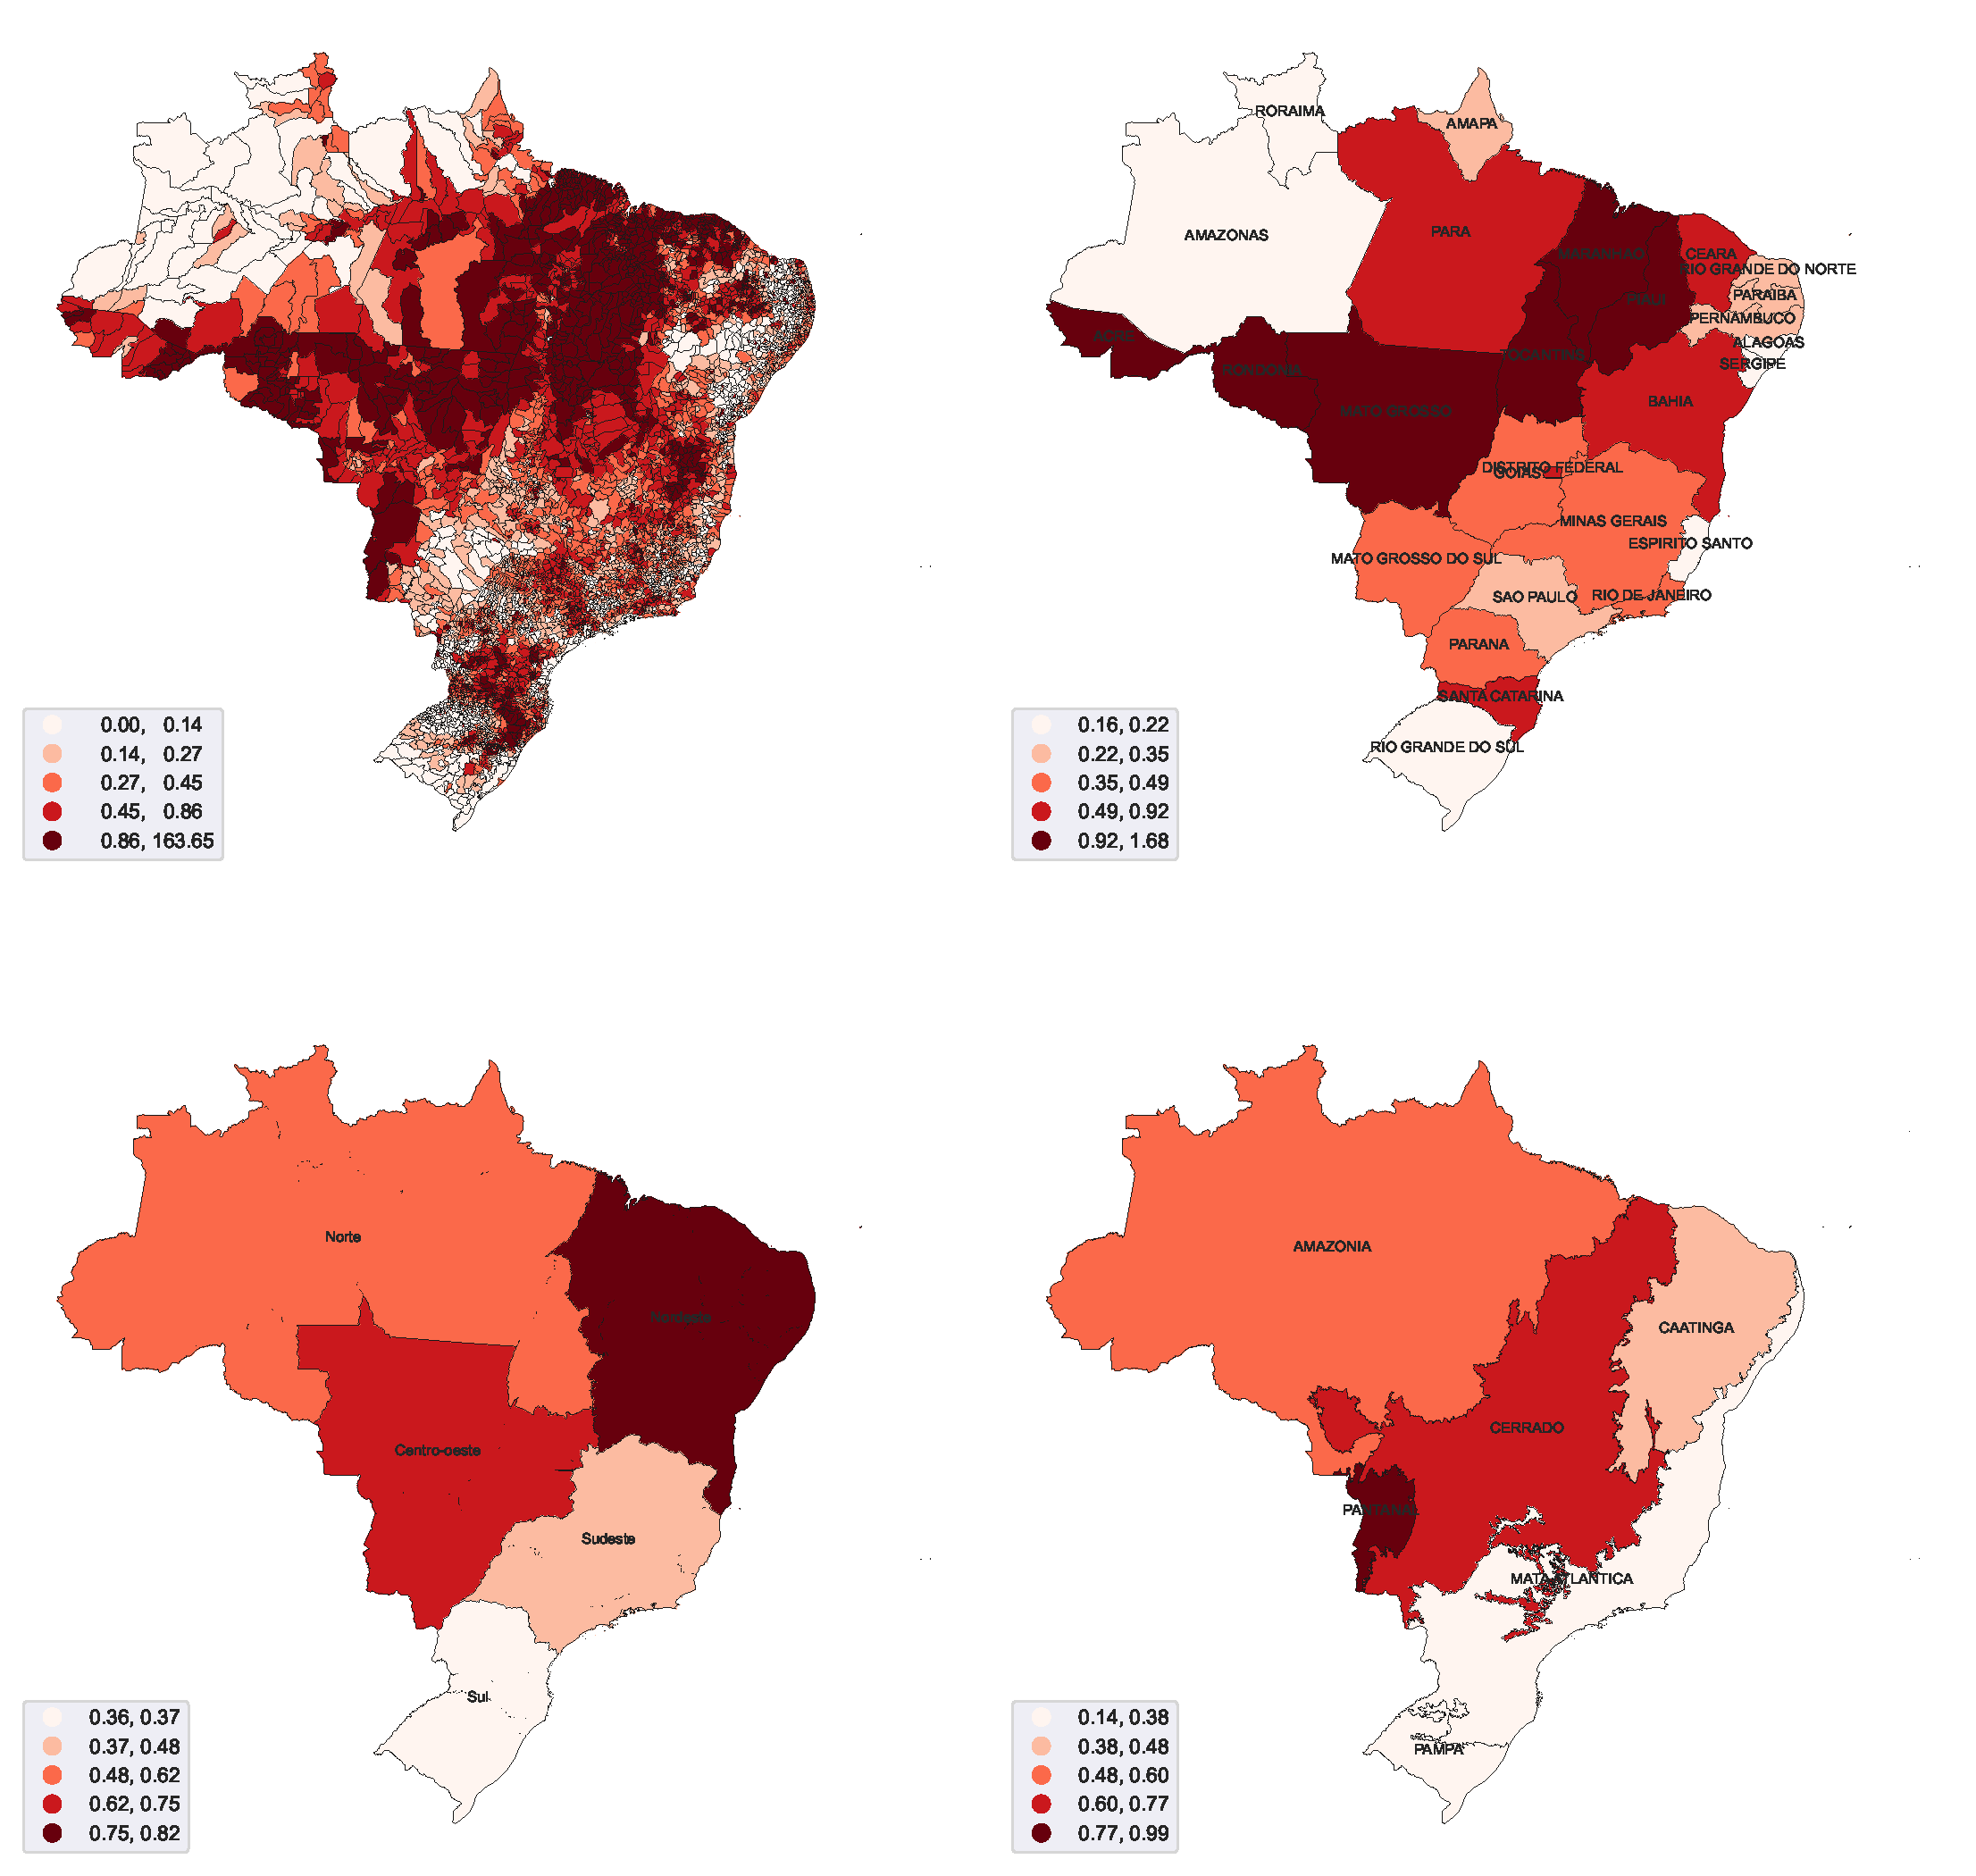
\includegraphics[width=25em]{brasil_focos}
    \end{center}
    \legend{Fonte: O Autor}
    \label{fig:brasil_focos}
\end{figure}

A Figura \ref{fig:brasil_focos} é fruto da relação dos dados de focos de queimadas com dados geográficos do país proveniente do IBGE. Nela é apresentado a quantidade de focos por $km^2$ para cada minicípio, estado, região e bioma do país desde o início dos dados do satélite de referência. A quantificação não é fixa para todos dos mapas, por isso cada mapa possui uma legenda que fica no canto esquerdo inferior. Cada linha da legenda representa o valor inicial (exclusivo, exceto no primeiro) e o valor final (inclusivo) do intervalo. 

O bioma Pantanal, apesar de apresentar queimadas mais recentes, já se destaca como o bioma que teve mais focos detectados, quase um foco por $km^2$. Logo depois vem o Cerrado, bioma de interesse de vários trabalhos que envolvem as queimadas, com a maior concentração de focos na parte superior de bioma, onde se intersecta com a região Norte e Nordeste. Os biomas Pampa, Mata Atlântica e Caatinga apresentam a menor proporção de focos por $km^2$, provalmente por já estarem muito degradados pelo processo de urbanização que começou na costa do país.

Pará, Rondônia e Acre são estados que apresentaram bastante focos e são cobertos quase completamente pelo bioma da amazônia. Por outro lado, estados nessa mesma situação, como Amazonas, Roraima e Amapa tem poucos focos. Muitas cidades do nordeste do Rio Grande do Sul e Santa Catarina também se destacaram, apesar da região Sul inteira não apresentar valores significativos. 

Por fim, com essa exploração inicial dos dados de focos do INPE, ficou claro que o tema ainda é bem relevante atualmente. Só no ano de 2022 foram detectados mais de 4.5 milhões de focos e mais da metade desses no bioma da Amazônia. O tema das queimadas no país é algo que precisa de atenção e de políticas públicas direcionadas às áreas que risco. A importância do tema, somado a alta cobertura de satélites produzindo dados públicos sobre os focos diariamente, fomenta o desenvolmento de novos métodos de análise automática desses dados.

\section{Detecção de focos ativos e área queimada}
\label{sec:deteccao_focos_section}

Nesta seção é abordada de forma mais detalhada como os dados brutos dos sensores dos satélites são usados de fato para encontrar focos ativos de queimadas e como o cálculo da área queimada é realizado atualmente. O texto começa com uma explicação de como funciona o processamento dos dados brutos e depois apresenta o método mais consolidado atualmente de detecção de focos ativos. Em seguida, são apresentados quatro métodos diferentes para o cálculo da área queimada, sendo dois mantidos pelo INPE, outro pela NASA e outro pela ESA. 

Os dados brutos dos sensores dos satélites são processados usando algoritmos específicos e produzem resultados chamados de ``produtos''. Nesse processo, os algoritmos corrigem distorções, eliminam ruídos e convertem os valores para dados que podem ser representados visualmente. Os produtos podem ter várias finalidades, como detecção de níveis de $CO_2$, radiância do solo, anomalias térmicas, entre outros, além de servirem como entrada para outros produtos. Os produtos podem ser classificados pelo seu nível de maturidade, como apresentado na Tabela \ref{table:nivel_maturidade_produtos}, e pelo nível de processamento dos dados, como listado na Tabela \ref{table:nivel_processamento_produtos}.

\begin{table}[htbp]
\centering
\caption{Nível de maturidade dos produtos}
\begin{tabular}{ @{}lp{12cm}@{} }
  \toprule
  \textbf{Nível} & \textbf{Descrição} \\
  \midrule
  Beta & Apenas deve ser usado para testes \\
  Provisório & O produto está em melhoria e segue sendo validado, não há garantias de qualidade \\
  Validado & O produto tem alta qualidade e pode ser usado para estudos rigorosos, como de mudanças climáticas. É subdividido em 4 estágios de validação. Nessa fase, o produto ainda pode seguir melhorando para atingir estágios mais altos de validação \\
  \bottomrule
\end{tabular}
\legend{Fonte: O Autor com base em \citep{maturiryLevelsNasa}}
\label{table:nivel_maturidade_produtos}
\end{table}

\begin{table}[htbp]
\centering
\caption{Nível de processamento dos dados dos produtos.}
\begin{tabular}{ @{}lp{12cm}@{} }
  \toprule
  \textbf{Nível} & \textbf{Descrição} \\
  \midrule
  Nível 0 & É o mais próximo dos dados brutos, com tratamento apenas de erros gerados pela comunicação dos dados, como dados duplicados \\
  Nível 1 & São dados georeferenciados com correções geométricas em relação a superfície da terra. Contém dados como radiância e reflectâncias. São subdivididos entre 1A, 1B e 1C \\
  Nível 2 & São dados referentes a geofísica da terra, como características da superfície terrestre, dados atmosféricos, níveis de poluentes, entre outros. São subdivididos entre 2A e 2B \\
  Nível 3 & São dados de nível 2 organizados no espaço e agrupados em perídos de tempo fixo (diário, mensal, anual), permitindo uma análise em escala global. \\
  Nível 4 & Envolve o uso dos dados em modelos ou uso deles em conjuntos com outros dados ou produtos, produzindo estimativas mais aprimoradas \\
  \bottomrule
\end{tabular}
\legend{Fonte: O Autor com base em \citep{dataProcessLevel}}
\label{table:nivel_processamento_produtos}
\end{table}

A evolução dos produtos gerados a partir do sensor MODIS é contínua à medida que a série temporal se expande. Isso resulta em diferentes versões do conjunto de produtos, denominado ``Collection'' e seguido por um número que define a versão. Por exemplo, a versão mais recente atualmente é a Collection 6.1, que também pode ser referida de forma simplificada como C6.1. Durante o desenvolvimento de uma nova versão, a versão anterior continua disponível enquanto os cálculos e processamentos são atualizados para os diferentes produtos. Isso permite que os usuários tenham acesso contínuo aos dados e resultados até que a nova versão esteja completa. A Tabela \ref{table:versoes_collection} apresenta um resumo das principais mudanças que ocorreram de uma versão para outra do Collection, começando pela versão que surgiu no mesmo ano do lançamento do satélite AQUA.

\begin{table}[htbp]
\centering
\caption{Versões resumidas do Collection para o sensor MODIS.}
\begin{tabular}{ @{}lllp{10cm}@{} }
  \toprule
  \textbf{Versão} & \textbf{Criação} & \textbf{Fim} & \textbf{Descrição} \\
  \midrule
  4   & 2002 & 2006  & Primeira versão que atinguiu 3 estágios de validação \\
  5   & 2005 & 2016  & Primeira grande coleção científica, que foi amplamente distribuída. \\
  5.1 & 2008 & 2016  & Atualização fundamental para o Produto L2 de Aerossol (04\_L2) e o Produto L2 de Nuvem (06\_L2) - juntamente com todos os produtos L3 para incorporar as atualizações do L2. \\
  6   & 2013 & 2018  & A Coleção 6 incluiu muitas novas atualizações científicas e melhorias. \\
  6.1 & 2017 & Atual & Corrigiu problemas nos dados de entrada do Nível-1B (L1B) - com algumas novas melhorias nos produtos do Nível-2 (L2) e Nível-3 (L3) adicionadas. \\
  \bottomrule
\end{tabular}
\legend{Fonte: Traduzido e modificado a partir de \citep{modisCollectionVersions}}
\label{table:versoes_collection}
\end{table}

\subsection*{Produtos de focos ativos}

Os algoritmos que geram produtos de focos ativos, geralmente usam diferentes canais dos sensores dos satélites, entre a luz visível e o infravermelho, e podem ter comportamentos distintos dependendo se a imagem foi gerada à noite ou de dia. Podem também usar limiares dinâmicos, de acordo com a região do planeta, que são calculados, com base em uma espécie de média das temperaturas nas regiões próximas ao longo dos dias. Além disso, é comum a aplicação de máscaras para eliminar regiões submersas, costeiras, desérticas e que estavam nubladas na hora da passagem do satélite empregado.

Para simplificar o trabalho, apresentamos apenas o método empregado para a detecção de focos ativos oficial da NASA, a partir do sensor MODIS \citep{GIGLIO2016}, que faz parte de Collection 6.1. O método recebe como entrada os produtos Nível 1B de radiância dos dois satélites (MOD021KM/MYD021KM) e os produtos Nível 1A (MOD03/MYD03) que identificam regiões de água, regiões costeiras e de terra. O resultado são dois produtos de Nível 2 e de resolução espacial 1Km, MOD14 para o satélite Terra e MYD14 para o satélite Aqua.

O processamento começa identificando e eliminando as regiões costeiras dos dados de reflectância, a fim de evitar confundir áreas terrestres mais quentes com áreas de água. Em seguida, ocorre a filtragem das regiões com cobertura de nuvens, utilizando limites atualizados, com cuidado para não excluir regiões de fumaça proveniente de incêndios ativos. As regiões remanescentes passam por um processo de avaliação para determinar potenciais píxels de fogo ativo. Esse processo envolve o teste da reflectância em relação a limiares dinâmicos, que são constantemente atualizados e ajustados para diferentes regiões do planeta, no caso das áreas terrestres. Para regiões onde não há dados suficientes para calcular os limiares dinâmicos ou para áreas de água, é utilizado um limiar fixo igual ao do Collection 5.

O algoritmo passa então a calcular médias de reflectância em uma grade centrada no pixel potencial de fogo ativo. Com base nessas médias locais, os pixels que atendem aos diversos testes relacionados a essas médias são selecionados. Os pixels que não possuem dados suficientes na vizinhança e não passaram nos testes são rotulados como ``sem dado''. Em seguida, o algoritmo entra em uma fase de descarte dos pixels preliminarmente classificados como fogo ativo, a fim de reduzir os falsos positivos. Durante essa fase de descarte, os pixels são eliminados se forem identificados reflexos solares maiores do que o aceitável ou se estiverem próximos a regiões costeiras, tanto para pixels na água quanto na terra. Além disso, outros filtros são aplicados exclusivamente para pixels em terra: se eles pertencem a regiões desérticas ou se estão em regiões de clareiras florestais.

O INPE empregava seu próprio algoritmo de detecção de focos de queimadas para o sensor MODIS, o qual produzia dados de maior confiabilidade \citep{PerguntasFrequentesINPE}. No entanto, a partir de 2017, o instituto adotou também os algoritmos do Collection 6 e reprocessou toda a sua base de dados de focos de queimadas. Isso marcou o início da chamada Base 2 de queimadas, que é totalmente compatível com os produtos de queimadas da NASA \citep{PerguntasFrequentesINPE}. Anteriormente, quando o Collection 5 estava em uso, eram observados falsos positivos em clareiras florestais e falsos negativos para grandes queimadas que estavam obscurecidas por fumaça densa \citep{SCHROEDER2008}, o que justificava o desenvolvimento de um algoritmo próprio pelo INPE para o Brasil. Como esse algoritmo  não é mais utilizado e seus resultados foram substituídos na base de dados do INPE, ele não é abordado neste trabalho.

\subsection*{Produtos de área queimada}

Nesta parte, são apresentados alguns dos produtos mais consolidados para o cálculo de área queimada no Brasil e no mundo: AQ1Km, AQ30m, MCD64A1 e FireCCI51. Um resumo desses quatro produtos pode ser encontrado na Tabela \ref{table:resumo_produtos_area_queimada}. A tabela fornece informações do nome do produto, o ano de início de uso, a resolução espacial e temporal, os satélites utilizados no cálculo e a principal referência teóricas que embasam esses métodos. Além desses produtos, existem muitos outros trabalhos que abordam o cálculo de área queimada, e alguns deles são mencionados na Seção \ref{sec:trabalhos_relacionados}. 

\begin{table}[htbp]
\centering
\caption{Resumo dos produtos de área queimada.}
\begin{tabular}{ @{}llllll@{} }
  \toprule
  \textbf{Nome} & \textbf{Ano} & \textbf{Res. esp.} & \textbf{Res. tem.} & \textbf{Satélites} & \textbf{Embasamento teórico} \\
  \midrule
  AQ1km & 2015 & 1km & mensal & Aqua/Terra & \citet{libonati2015algorithm} \\
  AQ30m & 2014 & 30m & quinzenal & Landsat-8 & \citet{melchiori2014landsat} \\
  MCD64A1 & 2016  & 500m & mensal & Aqua/Terra & \citet{GIGLIO201872} \\
  FireCCI51 & 2018 & 250m & mensal & Aqua/Terra & \citet{Lizundia2020} \\
  \bottomrule
\end{tabular}
\legend{Fonte: O Autor}
\label{table:resumo_produtos_area_queimada}
\end{table}

Os algoritmos utilizados para calcular a área queimada empregam índices que são sensíveis à vegetação queimada, aplicados aos produtos de reflectância dos satélites. Atualmente, os mais utilizados envolvem uma combinação das bandas do infravermelho próximo (NIR: $0,78-1,2\mu m$) e do infravermelho de onda curta (SWIR: $1,2-3,0\mu m$), enquanto o uso do infravermelho de onda média (MWIR: $3-8 \mu m$) é menos comum. Estudos indicam que, em uma área queimada, a reflectância do NIR é reduzida e a reflectância do SWIR é aumentada, devido à queima da vegetação e à secura do ambiente, respectivamente \citep{CHUVIECO201945}. Esse comportamente é ilustrado na Figura \ref{fig:reflectancia_espectral}.

\begin{figure}
    \caption{Variação da reflectância (\%), no eixo y, em relação à frequência da luz eletromagnética emitida por uma floresta, no eixo x. A cor verde representa a reflectância de uma vegetação não queimada, a cor vermelha representa a reflectância do fogo ativo na parte inferior da floresta (no solo), a cor preta representa um incêndio na copa das árvores e a cor cinza representa a reflectância de uma vegetação queimada (carvão).}
    \begin{center}
        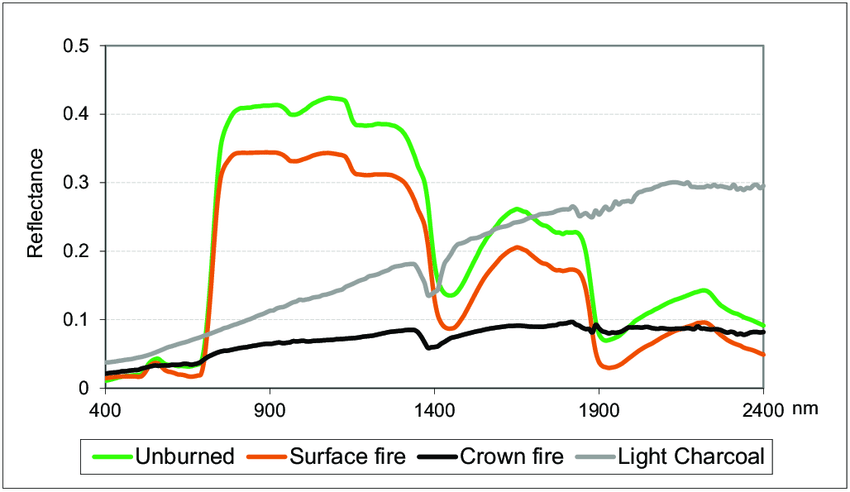
\includegraphics[width=25em]{Reflectance-spectra-for-unburned-vegetation-canopy-and-fires-affecting-different}
    \end{center}
    \legend{Fonte: Extraído de \citet{CHUVIECO201945} com base nos modelos Prospect + Geosail}
    \label{fig:reflectancia_espectral}
\end{figure}

O INPE utiliza dois produtos principais para a detecção de áreas queimadas: o AQ30m e o AQ1km. O produto AQ1km, desenvolvido em parceria com o Laboratório de Aplicações de Satélites Ambientais (LASA) do Departamento de Meteorologia da UFRJ, possui uma resolução espacial de 1 km e fornece dados diários agrupados em períodos mensais \citep{SiteAQ1km}. Por outro lado, o produto AQ30m possui uma resolução espacial de 30 metros e fornece dados quinzenais. Ambos os produtos são complementares e permitem uma análise abrangente das áreas queimadas. O AQ1km é adequado para avaliações mais amplas, como a determinação da porcentagem de área queimada em todo o Brasil durante um mês específico. Já o AQ30m fornece dados locais mais precisos, embora muitas regiões do Brasil não são processadas ou os dados não estão disponíveis publicamente.

O produto AQ1Km está em fase provisória de desenvolvimento (conforme Tabela \ref{table:nivel_maturidade_produtos}). É derivado de dados coletados pelo sensor MODIS, utilizando simultaneamente os satélites Aqua e Terra, além de incorporar informações de focos de queimada do INPE de diferentes satélites \citep{libonati2015algorithm}. Resumidamente, o algoritmo do AQ1km inicia filtrando os dados de reflectância com base em critérios de cobertura de nuvens e posição espacial para minimizar distorções. Em seguida, os dados são agrupados por mês para preencher eventuais lacunas diárias. O algoritmo identifica as áreas denominadas ``HotSpots'' (pontos quentes), que correspondem a regiões com atividade de fogo durante o período analisado. Posteriormente, é calculado um índice de vegetação para essas áreas, utilizando dados de reflectância no infravermelho próximo (NIR) e no infravermelho de onda média (MWIR), conforme proposto em \citet{libonati2011}, comparando-o com o mesmo índice do mês anterior. Por fim, são identificadas regiões próximas às áreas classificadas como queimadas no passo anterior, mas que não apresentaram um indicador suficientemente forte, podendo indicar que ocorreu uma queimada parcial ou que a intensidade do fogo foi baixa naquela localidade.

O produto AQ30m é gerado a partir de imagens do satélite Landsat-8, utilizando a diferença entre os índices de vegetação NDVI (Normalized Difference Vegetation Index), NBRL (Normalized Burn Ratio) e BAI (Burned Area Index) entre imagens consecutivas \citep{melchiori2014landsat}. Esses dados passam por uma filtragem com base em limiares definidos por especialistas e, em seguida, são suavizados usando um filtro de mediana 3x3 para eliminar valores discrepantes. O passo final envolve a construção de polígonos com base nos valores calculados e a remoção de polígonos muito pequenos. A implementação desse produto foi feita em Python, utilizando algumas ferramentas de processamento de dados que este trabalho também utiliza (mais detalhes no Capítulo \ref{chp:implementacao_metodo}). 

No entanto, o processo atualmente não é totalmente automatizado e requer uma avaliação final de um especialista do instituto antes da divulgação. Isso é necessário pois a degradação da vegetação pode ter ocorrido por outro fator além da queimada, como desmatamento, colheita ou preparação do solo. Quando os especialistas não tem certeza se a área destacada foi originada por uma queimada, a classificação é de não-queimada. Em \citet{dosclassificaccao}, são apresentadas algumas técnicas de aprendizado de máquina aplicadas na avaliação automática desse produto, obtendo resultados promissores (ver a Seção \ref{sec:trabalhos_relacionados}).

A NASA também mantém um produto específico para o cálculo da área queimada, chamado de MCD64A1, utilizando também os dados dos dois satélites com sensor MODIS \citep{GIGLIO201872}, de resolução espacial de $500m$ e temporal de um mês. Diferente da versão anterior, a MCD45 (C5), esse algoritmo combina as detecções de fogos ativos de 1 km do Collection 6.1 (ver Seção \ref{sec:deteccao_focos_section}) com um índice de vegetação sensível a queimadas, construído a partir dos canais 5 e 7 do SWIR do sensor MODIS, capturando a reflectância característica do solo em áreas queimadas. A combinação dos dados de fogos ativos e do índice de vegetação permite que o algoritmo se adapte às diferentes regiões e ecossistemas em todo o mundo. Os artefatos produzidos pelo produto podem ser baixados gratuitamento para cada mês a partir de novembro do ano de 2000 pelo site da Earthdata (\url{https://urs.earthdata.nasa.gov}).

O algoritmo inicia selecionando os dados diários de reflectância válidos, ou seja, dados que não contêm nuvens, fogo ativo, estão localizados em terra e possuem valores dentro do intervalo de 0 a 1. Em seguida, calcula o Índice de Vegetação (IV) para cada célula da grade. Posteriormente, o algoritmo calcula a diferença estatística do IV (S), comparando uma janela de dados de 8 dias antes e 8 dias depois do período avaliado. As regiões que não possuem dados confiáveis dentro dessas janelas de tempo são marcadas como não classificadas. Os dados passam por uma classificação inicial utilizando as estatísticas de S e outras informações de probabilidade de queima. Por fim, o algoritmo analisa as regiões vizinhas às que foram previamente classificadas como queimadas, aplicando uma fórmula probabilística que utiliza dados de focos ativos nessas regiões.

A ESA desenvolveu o FireCCI51, um produto avançado para o cálculo de áreas queimadas \citep{Lizundia2020}. Esse produto representa uma evolução em relação aos produtos anteriores, FireCCI41 e FireCCI50. Assim como o MCD64A1, o FireCCI51 combina detecções de focos ativos e dados de reflectância NIR do sensor MODIS, porém com uma resolução mais refinada de 250m. O algoritmo do FireCCI51 é dividido em duas fases principais. Na primeira fase, chamada de ``semente'', são coletados os pontos com alta probabilidade de terem sido queimados. Esses pontos são selecionados com base nas detecções de anomalias térmicas (focos ativos) e na diminuição do NIR, que é um indicativo de área queimada \citep{pereira1999}. Em seguida, o algoritmo passa para a fase de ``crescimento'', na qual são aplicados limiares locais a partir das sementes para identificar completamente as áreas queimadas. Posteriormente, é realizada uma poda para eliminar áreas que cresceram muito além das sementes iniciais, utilizando heurísticas que visam reduzir os falsos positivos.

\section{Trabalhos Relacionados}
\label{sec:trabalhos_relacionados}

Muitos outros trabalhos antes deste versaram sobre os dados de queimadas e, em menor escala, especificamente sobre o cálculo das áreas queimadas. Além dos trabalhos fundamentais, mencionados na Seção \ref{sec:deteccao_focos_section}, que deram origem aos produtos AQ1Km, AQ30m, MCD64A1 e FireCCI51, realizados por \citet{libonati2015algorithm}, \citet{melchiori2014landsat}, \citet{GIGLIO201872} e \citet{Lizundia2020}, respectivamente, são apresentados outros estudos que também inovaram no tema. São discutidos e apresentados os resultados obtidos por esses estudos e, ao final, são abordadas questões práticas e as características que tornam o presente trabalho único em relação aos demais.

O primeiro trabalho analisado é o \citet{dosclassificaccao} que se dedicou a eliminar a necessidade de uma avaliação humana no produto AQ30m, para o cálculo de áreas queimadas a partir de imagens do satélite Landsat-8. O documento aborda os resultados do treinamento de cinco modelos de aprendizagem de máquina: K-Nearest Neighbors (kNN), Decision Trees (DT), Random Forests (RF), Neural Networks (NN) e Support Vector Machines (SVM). São usadas quatro dados de entradas para esse modelo: Quantidade de queimadas anteriores próximas a área analisada, focos ativos de queima de diferentes satélites extraídos da base de dados do INPE, valor do índice Mid-Infrared Burn Index (MIRBI) e valor do índice Normalized Difference Water Index (NDWI).

O treinamento desses modelos foi com 9 imagens no período de 16/03/17 a 24/09/17 na região órbita-ponto 223/067. A validação foi feita com uma imagem em 10/10/17 e obteve resultado melhores nos modelos Random Forests e Redes Neurais. A acurácia geral ficou acima de 97\% para esses modelos. O modelos de K-Nearest Neighbors e Decision Trees ficaram entre 80\% e 90\% de acurácia. O pior modelo, o Support Vector Machines, obteve acurácia de pouco mais de 50\%. O trabalho conclui que os modelos podem atingir boas acurácias, mas como são treinados usando modelos de classificação, ao final o resultado é sempre uma classificação binária entre ``Queimado'' e ``Não queimado''. Isso simplifica muito o treinamento dos modelos, mas pode não ser ideal por agrupar áreas de desmatamento, colheita ou preparação do solo em uma classe errada.

O segundo trabalho analisado é o \citet{pereira2017burned} que usa um modelo de aprendizagem de máquina chamado de Máquina de Vetores de Suporte de Classe Única (OC-SVDD) para o mapeamento de áreas queimadas no Cerrado brasileiro com uma resolução de 300m. O método precisa apenas de dados da classe ``Queimada'', o que simplifica sua automatização. Para alimentar o modelo, foi usado dados pré processados de focos ativos detectados pelo sensor VIIRS (resolução de 375m) representando a classe ``Queimada''. Junto aos focos, também foram usados dados quizenais de reflectância do satélite PROBA-V (missão da ESA descontinuada em 2020), com o intuito de detectar regiões queimadas que não foram indicadas pelos dados dos focos ativos, o que reduz o erro de omissão. Devido ao uso dos dados do PROBA-V o método recebeu o nome de AQM-PROBA.

O método foi avaliado contra o produto AQ30m e comparando os resultados com o MCD64A1 aplicados em 13 orbitas-ponto Landsat. A abordagem de avaliação é a mesma usada em \citet{libonati2015algorithm} e, consequentemente, neste presente trabalho, como dicutido na Seção \ref{sec:metodologia_avaliacao}. O AQM-PROBA apresentou em média 30\% de erros de omissão e 22\% de erros de comissão. Comparando com o MCD64A1, o método proposto indica mais queimadas verdadeiras, mas também aumenta a taxa de falsos positivos. A conclusão do trabalho é que o método AQM-PROBA produz resultados mais próximos da referência AQ30m comparado com o MCD64A1, mesmo que tanto o AQM-PROBA quanto o MCD64A1 subestimam a área queimada de referência.

\section*{Comparação e discussão}

Quanto aos produtos AQ1Km e MCD64A1, ambos utilizam dados do sensor MODIS para monitorar a reflectância da vegetação a fim de detectar áreas queimadas, embora tenham utilizado índices de vegetação diferentes. Os resultados apresentados pelo produto AQ1km em comparação com o MCD64A1 indicam muito mais áreas queimadas, mas apresentam uma menor acurácia geral. Em contraste ao MCD64A1, o produto AQ1km inova e se beneficia dos dados de diferentes satélites para definir as áreas de interesse e calcular o índice de vegetação. No entanto, ainda sofre das mesmas limitações do sensor MODIS, dependendo apenas de dois satélites, AQUA e TERRA, para o resultado final.

O produto AQ30m, embora tenha uma resolução espacial mais alta, possui algumas limitações em relação à sua disponibilidade e cobertura. A dependência de intervenção humana para a publicação final dos resultados pode atrasar a divulgação periódica dos dados no site do DGI, dependendo da disponibilidade da equipe do INPE. Além disso, a disponibilidade dos dados do satélite Landsat-8 nem sempre é garantida, podendo estar faltando ou corrompidos, o que impossibilita a derivação do produto. Outro aspecto é que a cobertura do produto não abrange todo o território nacional, ou pelo menos essa informação não é divulgada, abrangendo apenas algumas órbitas-ponto que incluem parte do Cerrado, parte de Rondônia e a região central da Bahia.

No caso do presente trabalho, não são utilizados os dados de produtos de reflectância dos satélites, como os produtos de infravermelho usados nos cálculos dos índices de vegetação dos trabalhos anteriores mencionados. Em vez disso, são utilizados apenas os dados de focos ativos provenientes de diferentes satélites processados pelo INPE. Isso simplifica o processo, uma vez que as considerações relacionadas a diferentes regiões e biomas do planeta já foram resolvidas no processamento dos focos ativos. Além disso, essa abordagem é mais resistente a falta de dados, pois se um ou mais satélites falharem, o método ainda será capaz de operar com os dados dos satélites restantes.


%%%%%%%%%%%%%%%%%%%%%%%%%%%%%%%%%%%%%%%%%%%%%%%%%%%%%%%%%%%%%%%%%%%%%%%%%%%%%%%


\chapter{Metodologia}

Neste Capítulo é abordado como o método utilizado para calcular as áreas queimadas foi desenvolvido. Começa com uma visão geral do método, depois entra em cada etapa de forma separada e mais detalhada.

\section{Visão geral da metodologia}

A metodologia desenvolvida visa calcular a área de vegetação queimada no Brasil, por meio da análise dos dados de focos de queimadas disponibilizados pelo INPE, juntamente com as características dos diferentes satélites e sensores. A premissa fundamental é que um foco de queimada detectado resulta em uma área queimada. Além disso, considera-se que a quantidade de focos detectados em uma determinada região, em um intervalo de tempo, está diretamente relacionada com a área efetivamente queimada na região. \par 

\begin{figure}[H]
    \caption{Diagrama do método. A entrada principal são os dados de focos de queimadas e a saída principal é a estimativa de áreas queimadas. Abaixo os resultados produzidos com a aplicação em um determinado local para cada estapa.}
    \begin{center}
        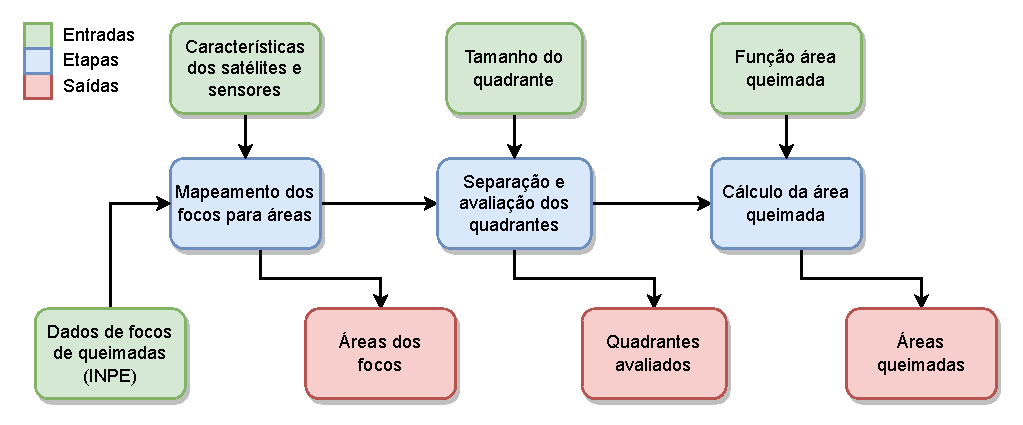
\includegraphics[width=35em]{metodologica_workflow}
        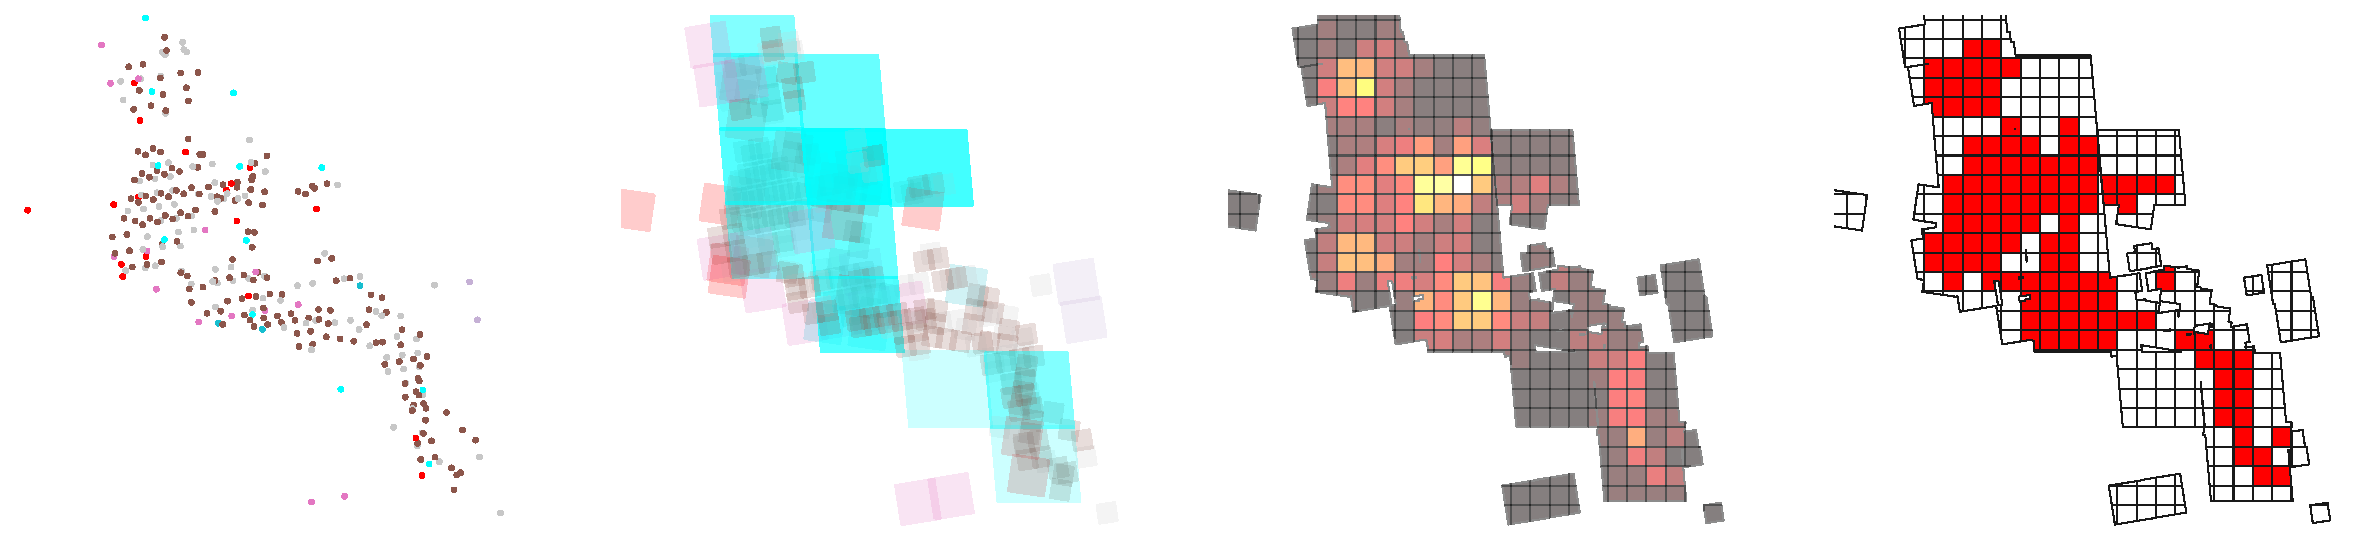
\includegraphics[width=35em]{exemplo_metodo_completo}
    \end{center}
    \legend{Fonte: O Autor}
    \label{fig:metodologica_workflow}
\end{figure}

O método completo, conforme apresentado na Figura \ref{fig:metodologica_workflow}, é composto por três principais etapas (cartões em azul): mapeamento dos focos para áreas, separação e avaliação dos quadrantes, e cálculo da área queimada. Cada etapa recebe dados de entrada e produz uma saída que, com exceção da última etapa, é usada como entrada para a etapa subsequente.

A primeira etapa transforma os pontos dos focos em áreas que representam a abrangência do foco. Essa etapa recebe dados de focos de queimadas do INPE, previamente filtrados para o intervalo de tempo de interesse, e produz como saída as áreas de cada foco. Essas áreas estão diretamente relacionadas às características do satélite e sensor que captaram a imagem original, como abordado na Seção  \ref{sec:deteccao_focos_section}, e, portanto, também precisam ser uma entrada para essa etapa.

Na segunda etapa, o espaço é dividido em quadrantes e avaliado. Esse passo recebe as áreas dos focos calculados na etapa anterior e o tamanho do quadrante, que pode ser definido pelo pesquisador. A saída são quadrantes com valores que representam a intensidade das queimadas ocorridas dentro de cada quadrante específico. A função de avaliação é proporcional à diversidade e quantidade das áreas de foco que intersectam os quadrantes.

Na terceira e última etapa, é realizado o cálculo das áreas queimadas, produzindo o resultado final do método. Essa etapa recebe como entrada os quadrantes avaliados no passo anterior e uma função de avaliação da área queimada, que pode ser definida pelo pesquisador. A função é aplicada a todos os quadrantes, resultando em um valor que representa a porcentagem provável de que a área do quadrante tenha sido queimada.

A Figura \ref{fig:metodologica_workflow} também ilustra a aplicação completa do método em uma área específica localizada no sudoeste do Pará, durante os dias 1 a 3 de setembro de 2022. Na primeira imagem, são mostrados os focos de queimada, sem nenhum tipo de pré-processamento. Na segunda imagem, os pontos são transformados em áreas. Em seguida, o espaço é dividido em quadrantes e avaliados. Na última imagem, o cálculo da área queimada considera todas as avaliações acima do valor 5 como quadrante totalmente queimado, resultando em uma área queimada de $33,32 km^2$.

O método é flexível e altamente configurável, podendo assim gerar resultados bem diferentes dependendo de suas entradas, ainda que para o mesmo conjunto de dados de focos. O pesquisador pode testar combinações de entradas e avaliar os resultados usando algum comparador (benchmark). Um exemplo seria compara as saídas do método com os resultado obtidos pelo produto AQ1km (abordado na Seção \ref{chp:trabalhos_relacionados}). Por fim, a aplicação do método bem como os resultados obtidos são abordados no Capítulo \ref{chp:resultados_discussão}.

\section{Mapeamento dos focos para áreas}

Quando um foco de queimada é detectado pelo INPE a partir de um satélite, o foco representa uma área quadrada aproximadamente do tamanho da resolução do sensor que capturou a imagem original. Ou seja, um foco dectado a partir de imagens do satélite AQUA, que utiliza o sensor MODIS, representa uma área de $\approx1Km^2$. Para um satélite com o sensor menos preciso, como o GOES-13, que utiliza o sensor GOES I-M com resolução espacial de $4Km$, a área representada seria 16 vezes maior, indicando uma menor precisão. \par

O cálculo exato da área coberta pelo foco deve levar em conta, além da resolução do sensor, as distorções provenientes dos seguintes fatores: Diferença de localização entre o foco e o satélite, e as caractísticas da órbita do satélite. No primeiro fator, quanto maior a distância entre os dois pontos, maior será a distorção em relação a área de corbertura do sensor. Para um satélite geoestacionário, por exemplo, essa distância é sempre muito grande, devido a sua órbita com altura de $36Km$ \citep{EmbrapaSatelites}. \par

No segundo fator, a inclinação dos satélites determinam como é a rotação da área coberta. Os satélites que orbitam a Terra em órbitas polares, possuem uma determinada inclinação que lhes permitem cobrir diferentes áreas de todo o planeta durante sua tragetória (Figura \ref{fig:orbita2022-08-10}). Quando o satélite está se movendo em uma trajetória ascendente, ou seja, do sul para o norte, a área coberta pelo sensor deve ser rotacionada em um sentido. Por outro lado, se a trajetória for descendente, do norte para o sul, a rotação deve ser no outro sentido. \par

\begin{figure}[H]
    \caption{Comparação entre pontos e áreas dos focos detectados pelo satélite Suomi NPP.}
    \begin{center}
        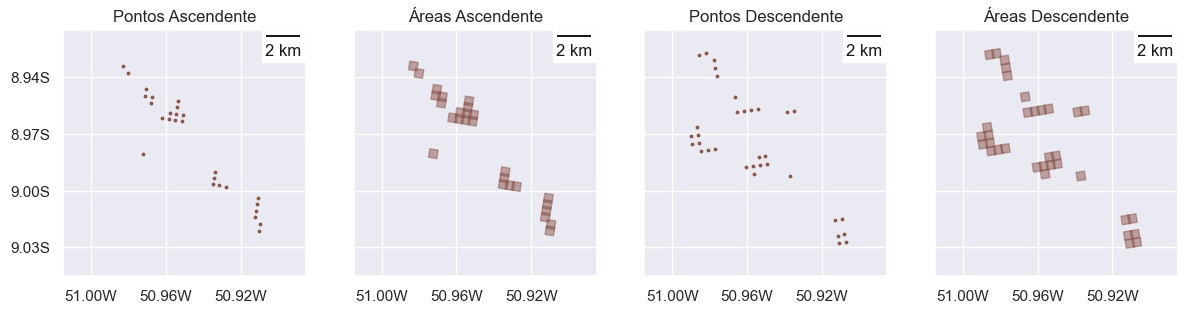
\includegraphics[width=35em]{comparacao_pontos_e_areas}
    \end{center}
    \legend{Fonte: O Autor}
    \label{fig:comparacao_pontos_e_areas}
\end{figure}

A Figura \ref{fig:comparacao_pontos_e_areas} apresenta dados coletados pelo satélite  Suomi NPP no dia dois de setembro de 2022. O primeiro par de imagens corresponde à órbita ascendente do satélite, enquanto o segundo par de imagens corresponde à órbita descendente. Observa-se que, na primeira e terceira imagens, os pontos dos focos de queimada estão alinhados, mas ligeiramente rotacionados em alguns graus, coincidindo com a inclinação do satélite. Na segunda e quarta imagens, os pontos ganham a área do sensor ($500m$) e encaixam perfeitamente entre seus vizinhos. A partir desse ponto até o final do documento, a área coberta pelo foco será chamada de medição. \par

\section{Separação e avaliação de quadrantes}

A separação entre quadrantes é a forma de discretizar os dados do espaço, que são contínuos. Os quadrantes abstraem os detalhes das medições dos diferentes satélites, com diferentes áreas e orientações. Como resultado, ilustrado na figura \ref{fig:satellite_quads_split}, temos uma grade regular que é usado para as operações de avaliação de serão descritas a seguir. \par

O tamanho do quadrante é uma entrada dessa etapa e pode ser definida pelo pesquisador. O valor recomendado desta entrada fica em torno de 0,004 a 0,005 graus, o que coincide com o tamanho da menor resolução de sensor presente nos dados, que é o VIIRS de 500m. \par

\begin{figure}[H]
    \caption{Separação entre quadrantes.}
    \begin{center}
        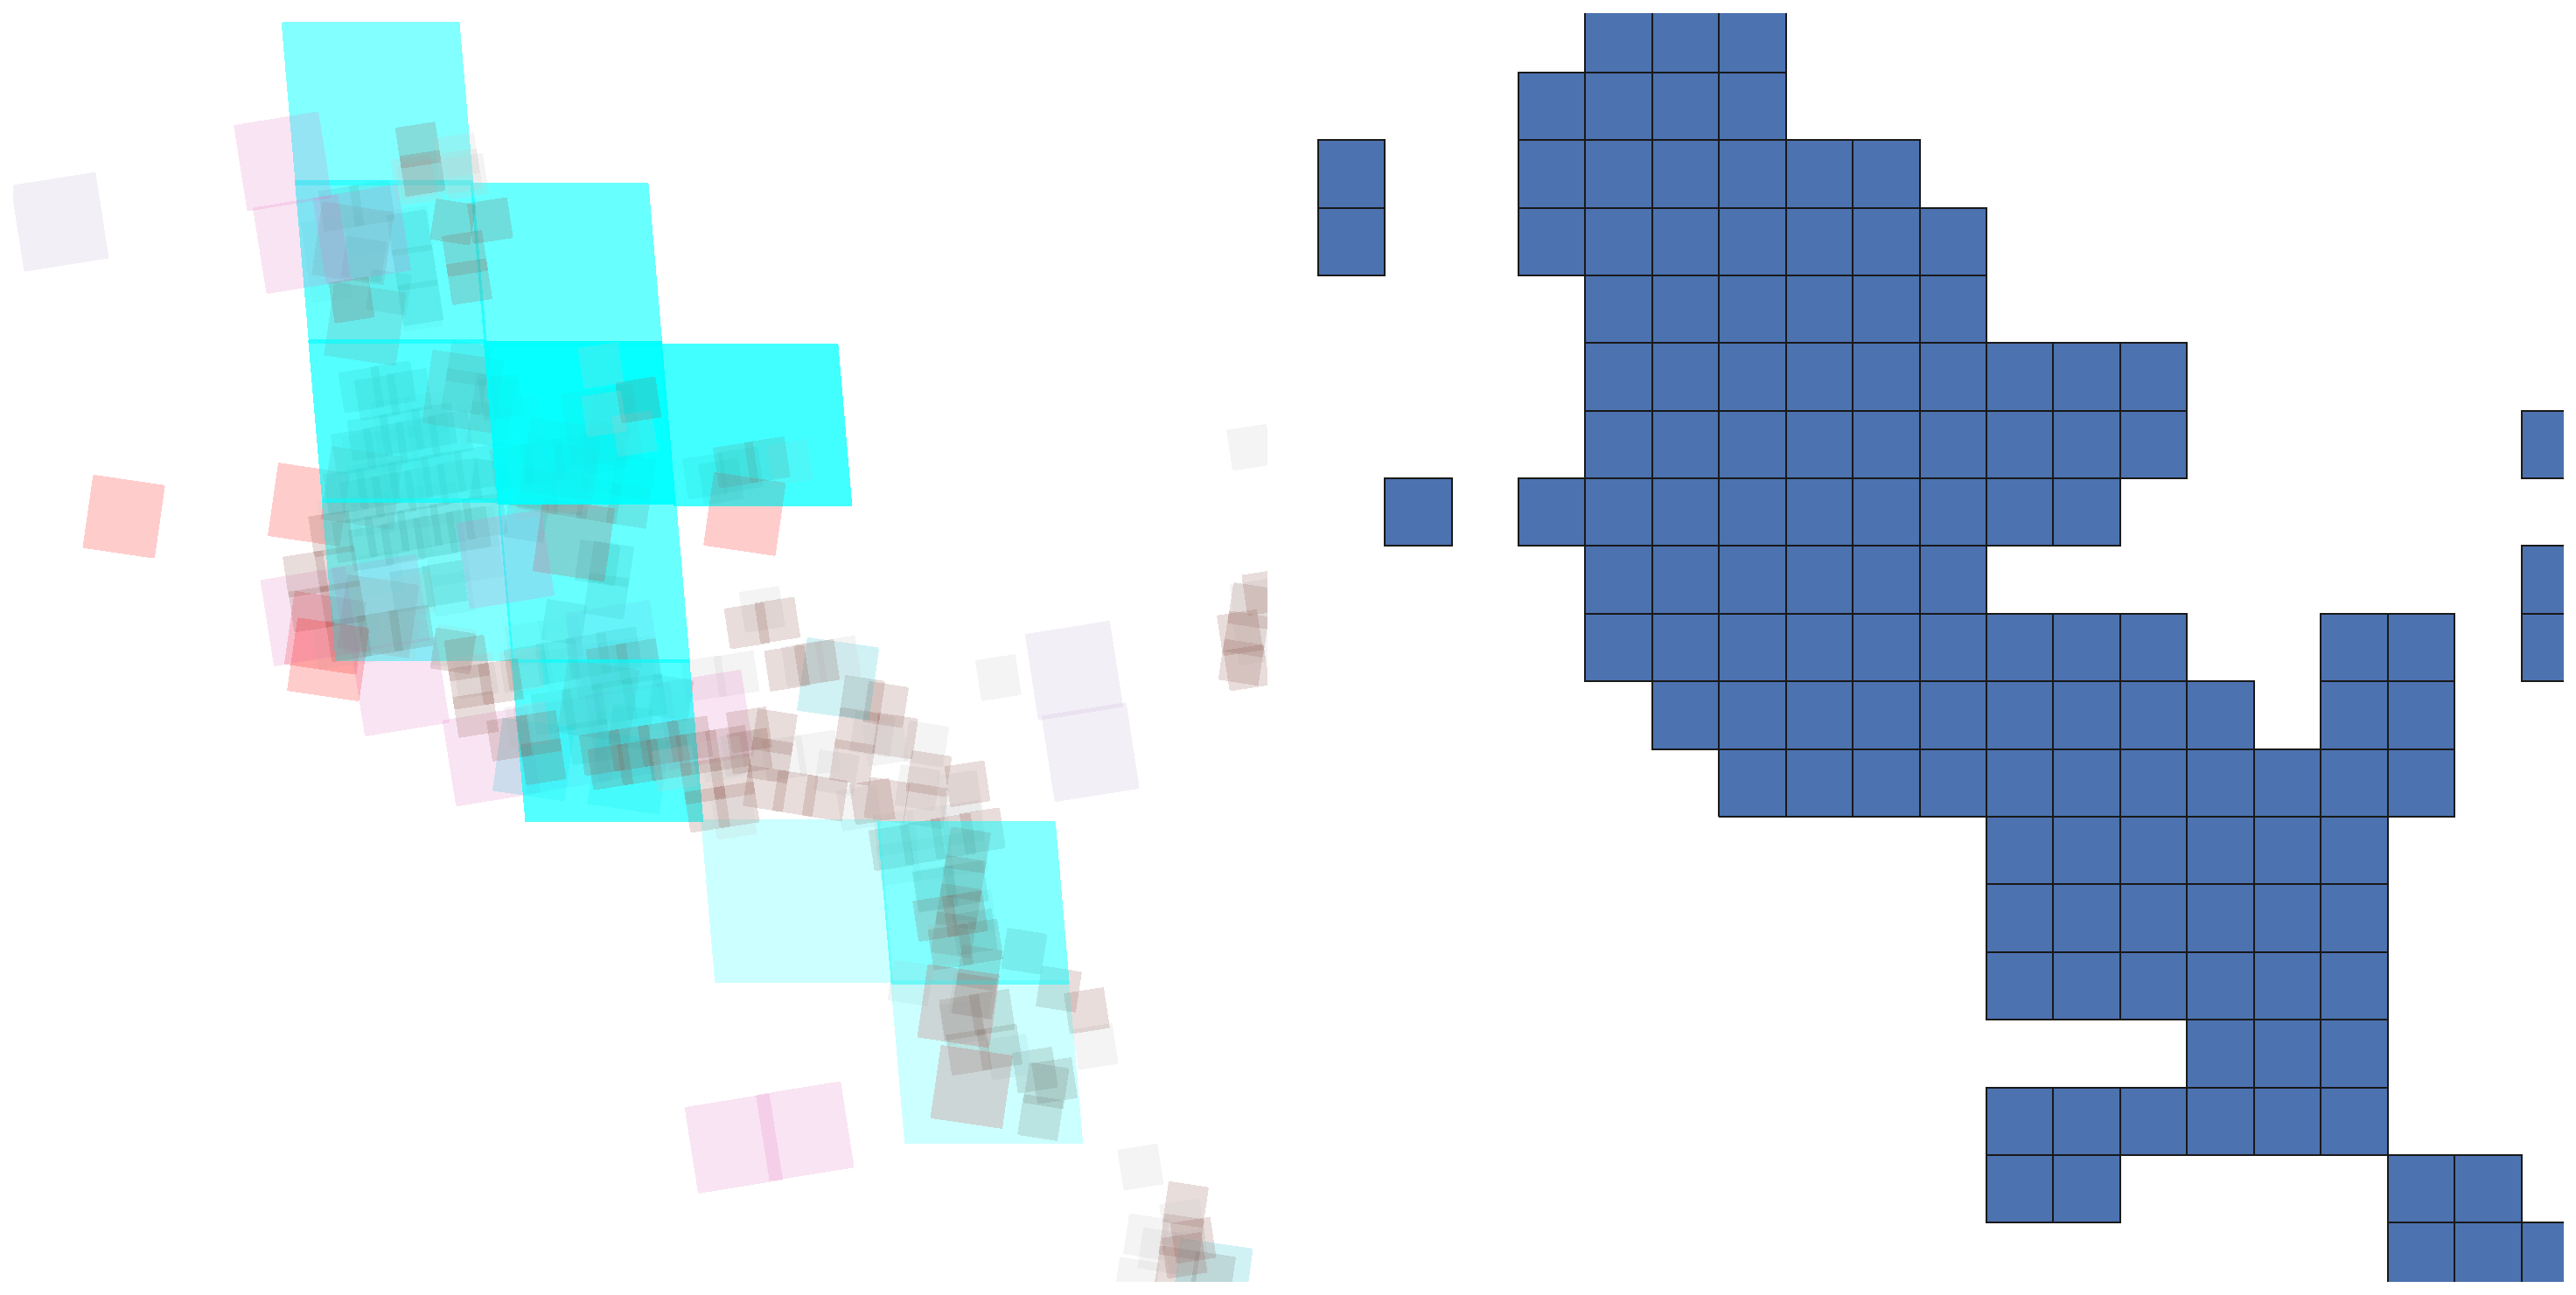
\includegraphics[width=20em]{satellite_quads_split}
    \end{center}
    \legend{Fonte: O Autor}
    \label{fig:satellite_quads_split}
\end{figure}

Com a distribuição dos quadrantes definida, é necessário atribuir a cada um deles um valor que represente a probabilidade de que a área contida tenha sido queimada. A avaliação dos quadrantes deve valorizar aqueles que apresentam medições de diferentes satélites. Essa abordagem justifica-se pelo fato de que ajuda a reduzir os ruídos nas medições e a identificar queimadas mais intensas. Além disso, diferentes satélites realizam medições em horários distintos (veja a Figura \ref{fig:tempo_medidas_satelites}), o que indica uma queimada mais prolongada. Em ambos os casos, queimadas mais intensas e duradouras sinalizam um maior potencial de o fogo se espalhar para outras áreas da vegetação. \par

Sendo $q$ o quadrante (polígono) a ser avaliado; $M$ um conjunto de todas as medições (área coberta pelo foco); operação $area(p)$ retorna a área de um polígono $p$ qualquer; operação $unique\_satelite(Q)$ retorna todos os satélites diferentes do conjunto $Q$; $min\_area$ é a área mínima de uma medição; $threshold\_satellite$ é o número mínimo de satélites para não ser penalizado. A definição formal da avaliação é dada por: \par

Para cada quadrante ($q$), é realizado o cálculo da intersecção com cada medição ($m$) contida nele, resultando em um conjunto $Qm$: \par

\begin{equation} \label{eqn:def_qm}
Qm = \{ m \in M \mid m \cap q \}
\end{equation}

Em seguida, é realizada uma filtragem no conjunto $Qm$, removendo todos os elementos que não possuem uma determinada área mínima, resultando em $Qm'$: \par

\begin{equation} \label{eqn:def_qm_line}
Qm' = \{ m \in Qm \mid area\left(m\right) \ge min\_area \}
\end{equation}

A partir de $Qm'$, é extraído o número de satélites diferentes presentes nesse conjunto, que é denominado $Us$: \par

\begin{equation} \label{eqn:def_us}
Us = \{ m \in unique\_satelite\left(Qm'\right) \}
\end{equation}

Além disso, é calculada a soma das áreas de $Qm'$ e dividida pela área total de $q$, resultando em $ia$. Ou seja, quantas vezes as áreas de $Qm'$ cabem dentro de $q$: \par

\begin{equation} \label{eqn:def_ia}
ia = \left(\sum_{m}^{Qm'} area\left(m\right)\right) \div area(q)
\end{equation}

Penalização de quadrantes que tenham poucos satélites diferentes, o valor de $c$ fica entre 0 e 1 e é linear. \par

\begin{equation} \label{eqn:def_c}
c = 1 - min\left(1, \frac{|Us|}{threshold\_satellite}\right)
\end{equation}

Finalmente, a avaliação final do quadrante ($aq$) é obtida pela expressão: \par

\begin{equation} \label{eqn:def_aq}
aq = |Us|^2 + ia - ai \cdot c
\end{equation}

A fórmula final \ref{eqn:def_aq} atribui um peso quadrático à quantidade de satélites diferentes presente no quadrante $q$. Isso garante que, à medida que a diversidade de satélites aumenta dentro do quadrante, o valor de $aq$ aumente de forma exponencial e se distaque dos demais quadrantes com menos diversidade. O resultado é somado com $ai$, que representa quantas vezes a área das medições somadas cabe no quadrante $q$. Esse termo impede que medições com pouca interseção dentro do quadrante tenham uma influência desproporcional no resultado final. \par

Além disso, há uma penalização aplicada aos quadrantes que apresentam poucos satélites diferentes. Quando a quantidade de satélites diferentes em um quadrante é maior do que um limite pré-estabelecido, chamado de $threshold\_satellite$, não há penalizações, ou seja, o valor de $c$ é igual a 0. Por outro lado, quando o quadrante não atinge o limite, uma parcela de $ai$ é descontada do resultado final. \par

Essa etapa é considerada concluída quando todos os quadrantes estão avaliados seguindo as equações apresentadas. Desta forma, a avaliação de um quadrante não depende de outras avaliações de seus vizinhos ou outra forma de dependência de dados, o que possibilita a avaliação paralela dos quadrantes. \par

\section{Cálculo da área queimada}

Finalmente, com os quadrantes avaliados, é possível estimar a área queimada para cada quadrante. É importante que o método de cálculo seja flexível, permitindo que o pesquisador teste diferentes métodos. Uma forma de fazer isso é atribuir um número que represente a porcentagem de área queimada dentro do quadrante e, em seguida, multiplicá-lo pela área total do quadrante para obter a área queimada dentro do quadrante. Após calcular a área queimada de cada quadrante, é necessário somar todos esses valores para obter a área total queimada. \par

Nesse sentido, o papel do pesquisador é definir uma função ($eval(v)$) que receba o valor do quadrante, calculado na etapa anterior, e retorne um número real entre zero e um. Essa função também pode receber o maior e o menor valor presente na avaliação dos quadrantes, valores que podem ser usados para normalizar o cálculo. Ou seja, o pesquisador pode definir uma função linear que indique que o quadrante só deve ser considerado totalmente queimado se o valor do quadrante for o maior.\par

Para facilitar o trabalho do pesquisador, a implementação pode fornecer funções embutidas comuns que definem a função $eval(v)$. Na Figura \ref{fig:eval_func_built_in}, são apresentadas algumas possibilidades de definições para essa função. A função mais simples é chamada de limiar, que estabelece que toda a área do quadrante deve ser considerada queimada se a avaliação for maior que um determinado valor e nenhuma área deve ser considerada queimada se não alcançar esse valor. Outra função simples é a linear, que faz o valor da área queimada crescer de forma linear dentro de um valor máximo e mínimo. A última função é a exponencial, semelhante à linear, mas com uma exponenciação que faz o valor crescer mais lentamente no início e de forma mais acentuada no final do intervalo. \par

\begin{figure}[H]
    \caption{Funções embutidas para cálculo de área.}
    \begin{center}
        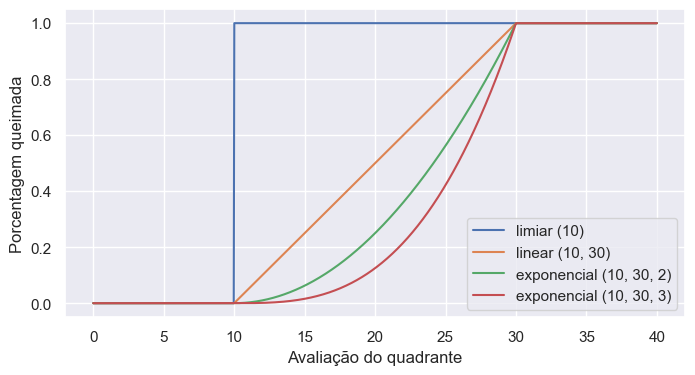
\includegraphics[width=25em]{eval_func_built_in}
    \end{center}
    \legend{Fonte: O Autor}
    \label{fig:eval_func_built_in}
\end{figure}

A Figura \ref{fig:aplicacao_funcoes_built_in} ilustra claramente como diferentes funções e parâmetros podem afetar significativamente os resultados na determinação da área queimada. Cada gráfico mostra a área queimada total calculada usando a função de área queimada indicada no título. Observa-se que a função limiar identifica mais áreas como queimadas, pois trata de forma igual os quadrantes com diferentes níveis de intensidade. No entanto, as funções exponenciais parecem mais próximas da realidade, já que consideram apenas uma porcentagem da área dos quadrantes próximos aos agrupamentos de alta intensidade como queimados. \par

\begin{figure}[H]
    \caption{Exemplo da aplicação das funções embutidas.}
    \begin{center}
        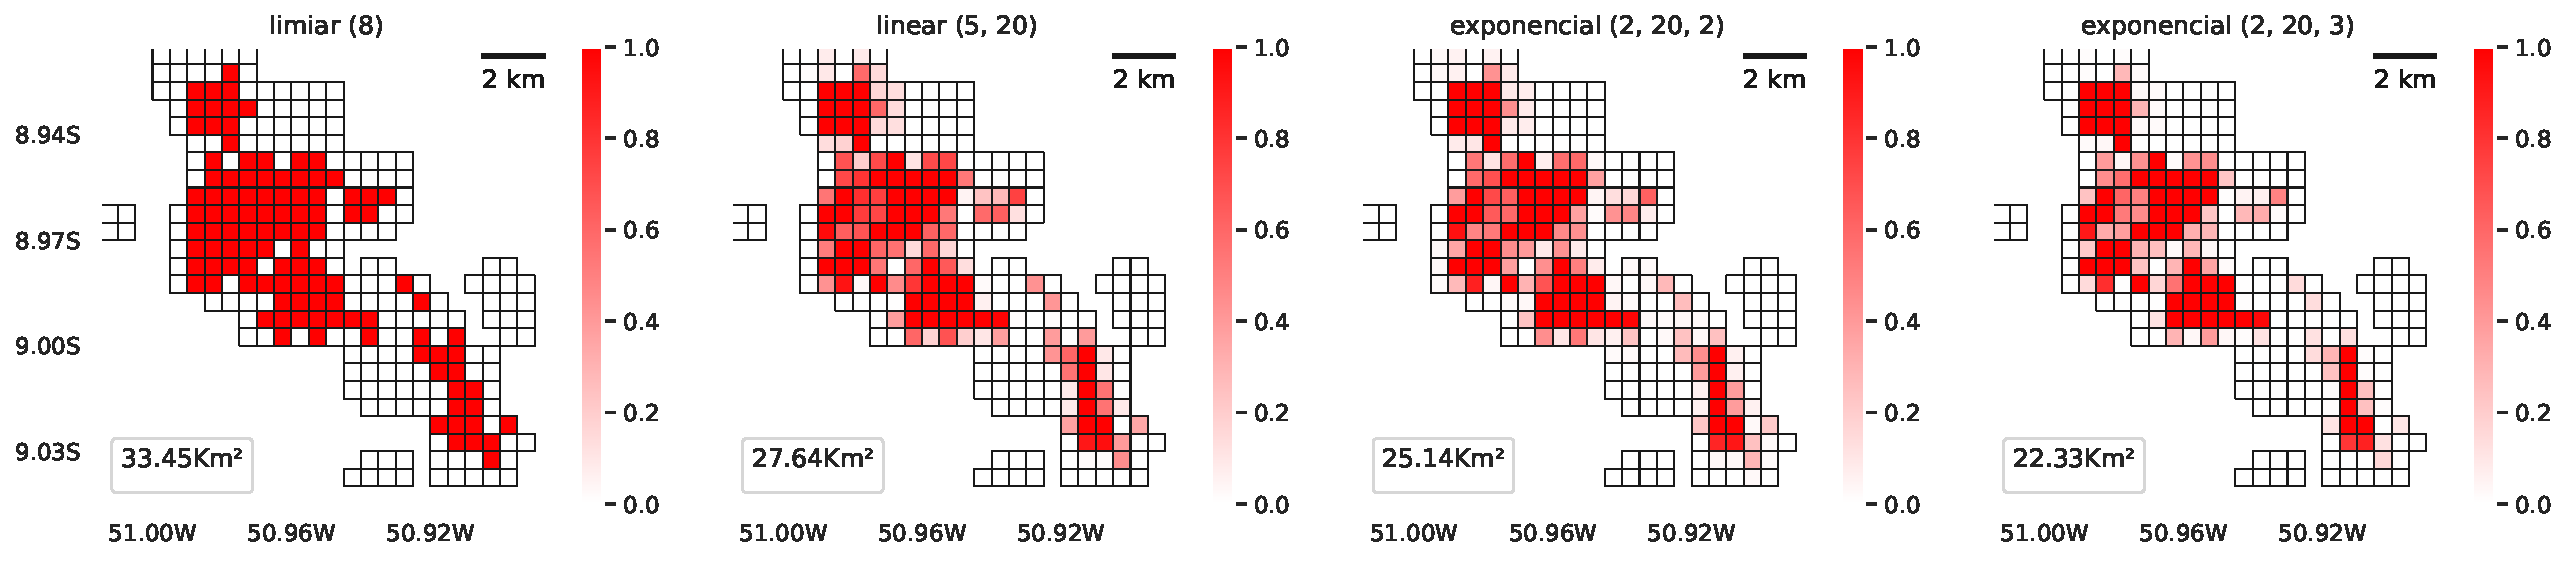
\includegraphics[width=35em]{aplicacao_funcoes_built_in}
    \end{center}
    \legend{Fonte: O Autor}
    \label{fig:aplicacao_funcoes_built_in}
\end{figure}

\chapter{Implementação do método}
\label{chp:implementacao_metodo}

Após a formalização do método de forma abstrata, esse Capítulo descorre sobre a implementação de fato do método. Primeiro está discutido como os dados do DBQueimadas foram coletados da base de forma automatizada. Em seguida, descorre-se sobre a implementação do método ....

\section{Coleta dos dados}

Uma parte fundamental do processo foi coletar os dados do site DBQueimadas, que é a fonte primária usada para cálculo das áreas queimadas. Para exportar os dados usando o navegador, é necessário preencher um formulário com os campos de data inicial, data final e um endereço de e-mail, com intervalo de tempo máximo um ano para cada pedido. Também é possível aplicar filtros ainda mais específicos, como continente, país, estado, município, satélite, bioma e unidades de conservação/terras indígenas. Após clicar em ``Exportar'', uma mensagem contendo um link de download é enviada para o e-mail informado, e o arquivo disponibilizado é um CSV compactado em formato zip.

Embora o site tenha boa usabilidade, seria impraticável baixar todos os dados do Brasil manualmente sem sobrecarregar os servidores no INPE. Por isso, foi necessário entender como a solicitação dos dados era processada pelo site e, assim, automatizar o download. Foi identificado que o site faz uma requisição GET para a API do DBQueimadas, localizada em \url{https://queimadas.dgi.inpe.br/queimadas/exportacaobdq/exportar}, passando os parâmetros  codificados em JSON da URL, incluindo os filtros, e-mail e formato de arquivo desejado. Um exemplo de uso dessa API por meio de uma chamada CURL pode ser encontrado no \ref{anexo:usoApiInpe}.

Para automatizar o processo, desenvolvemos um script em Python que solicitava os dados de cada 30 dias, totalizando 300 requisições desde 1998 até 2022. Para não sobrecarregar os servidores do INPE, adicionamos uma espera de um minuto entre as requisições. Além disso, implementamos um sistema de registro de requisições em arquivo, que armazenou o estado de cada uma delas, evitando requisições duplicadas e possibilitando a retentativa das requisições que falharam por algum motivo. O programa foi considerado concluído apenas quando todas as requisições contidas no registro estavam marcadas como concluídas.

Para concluir o processo, ainda era necessário fazer o download do arquivo por meio do link enviado por e-mail. Utilizamos o Google Scripts, uma ferramenta que possibilita escrever programas simples, utilizando uma linguagem semelhante a JavaScript, com integração aos serviços do Google (como o Gmail). O script era executado com um intervalo de dois minutos, varrendo todos os e-mails novos provenientes do DBQueimadas. Com ele, foi possível extrair o link de cada mensagem e, finalmente, salvar o arquivo de forma automatizada. 

Os dois scripts trabalharam de forma concomitantemente, funcionando como uma espécie de produtor e consumidor distribuído. Enquanto um requisitava os dados para do INPE, o outro vasculhava os e-mails e salvava o arquivo em uma pasta específica. Quando o primeiro script identificava (por meio do nome do arquivo) que a resposta já estava salva, marcava a requisição como concluída no registro. Caso uma requisição permanecesse por mais de 30 minutos no estado pendente, o script fazia uma nova solicitação aos servidores do INPE.

Todo o processo de investigação e recuperação dos dados levou cerca de uma semana. Todos os arquivos baixados ocupam pouco mais de 4 gigabytes de armazenamento em disco e, juntos, somam exatamente 43.782.758 linhas. Ao final, eles foram recompactados em um único arquivo zip (450 megabytes) que está disponível para download em \url{https://bit.ly/3IgHIXH}, independentemente dos servidores do INPE.

Também foi utilizado os dados públicos territoriais do Brasil provenientes do Instituto Brasileiro de Geografia e Estatística (IBGE) para gerar gráficos delimitados em municípios, unidades federativas e biomas. O processo de aquisição desses arquivos se deu diretamente no site do IBGE. Todos os arquivos baixados estão no formato Shapefile, que é o formato responsável por armazenar dados vetoriais geográficos.


\section{Implementação do método}

Para toda a implementação e análise dos dados, foram utilizadas diversas ferramentas do ecossistema Python para Data Science, tais como NumPy, Pandas e Matplotlib. Além disso, foram empregadas bibliotecas específicas para análise de dados geográficos, como GeoPandas, Pysal, Xarray e Shapely. Para garantir a reprodutibilidade das execuções e a organização do código, foi adotado o Jupyter Notebook. Todos o código e demais artefatos gerados durante o projeto podem ser encontrados em \url{https://github.com/josebraz/INPE-Queimadas}, disponibilizados sob a licença MIT. \par

A biblioteca GeoPandas, amplamente utilizada na implementação, é uma extensão do Pandas que adiciona uma coluna especial chamada 'geometry'. Essa coluna permite armazenar as coordenadas e o formato dos dados em um sistema de coordenadas pré-definido. Além disso, o GeoPandas integra-se à biblioteca Shapely, que é usada para realizar cálculos e operações em estruturas geométricas espaciais. Com o uso dessas bibliotecas, é possível executar operações avançadas da teoria dos conjuntos em elementos geométricos, como união, interseção, diferença, entre outras, além de calcular a área de qualquer polígono que represente uma área no espaço. \par

O GeoPandas também oferece suporte à operação de junção espacial (spatial join) de forma otimizada. O spatial join permite combinar diferentes conjuntos de dados com base em sua relação espacial, de maneira semelhante a uma junção em um banco de dados, porém levando em consideração a proximidade geográfica. É possível utilizar diferentes critérios de proximidade geográfica, como verificar se um ponto está dentro de um polígono ou determinar a interseção entre dois polígonos. No contexto da implementação, o spatial join é utilizado para obter todas as medições que intersectam cada quadrante (interseção entre dois polígonos), que é a principal informação usada para avaliar um quadrante. \par

Após a coleta de dados mencionada anteriormente, os dados foram carregados no Python e algumas otimizações nas estruturas foram realizadas. Os 300 arquivos das queimadas foram lidos pelo Pandas e concatenados em um único DataFrame. Foi necessário converter o fuso horário das datas, que estavam no formato UTC, para o fuso horário de Brasília, a fim de facilitar a compreensão dos gráficos para os usuários brasileiros. Além disso, as colunas de texto, como município, estado, país e satélite, foram convertidas em categorias, que são uma forma de enumeração disponível no Pandas. Essa conversão ajudou a reduzir o consumo de memória, uma vez que muitos valores repetidos ocorriam nessas colunas, ocupando 2 Gb em mémoria. \par

Para otimizar o processamento e a leitura dos dados, também foi utilizada a biblioteca Dask especializada no processamento paralelo e distribuído. Essa biblioteca oferece a capacidade de criar clusters locais ou se conectar a clusters remotos, permitindo o envio de tarefas completas para serem processadas pelo cluster. Além disso, o Dask possibilita a leitura dos arquivos de forma paralela, o que resulta em uma redução significativa no tempo de carregamento dos dados. Após o carregamento completo do DataFrame a partir dos arquivos CSV originais durante a primeira execução, foi criado um arquivo no formato H5 que contém os mesmos dados, mas com uma estrutura otimizada para permitir uma leitura mais rápida. Nas execuções subsequentes do programa, ao invés de carregar novamente os arquivos CSV, o programa fará a leitura desse único arquivo H5, resultando em um carregamento ainda mais rápido dos dados.  \par

Durante o pré-processamento dos dados, foram identificadas regras de nomenclatura especiais para alguns satélites. No caso dos satélites AQUA (AQUA\_M-T e AQUA\_M-M) e TERRA (TERRA\_M-T e TERRA\_M-M), a última letra indica o período do dia em que ocorreu a passagem do satélite, sendo ``M'' para Manhã e ``T'' para Tarde. Outros satélites, como Suomi NPP, NOAA-19, NOAA-18, NOAA-16, NOAA-15 e NOAA-12, podem apresentar a última letra do nome como ``D'' para Diurno. Com base nessa compreensão das regras de nomenclatura, foi possível criar uma nova coluna que fornece o nome simplificado dos satélites, facilitando algumas análises. Em comparação com a coluna original dos satélites, que tinha 32 valores possíveis, a nova coluna contém apenas 22 valores possíveis. Para cada satélite, foi escolhida uma cor única, conforme apresentado na Figura \ref{fig:cores_satelites}, que é utilizada em todos os gráficos apresentados neste documento. \par

\begin{figure}[H]
    \caption{Cores escolhidas para cada satélite.}
    \begin{center}
        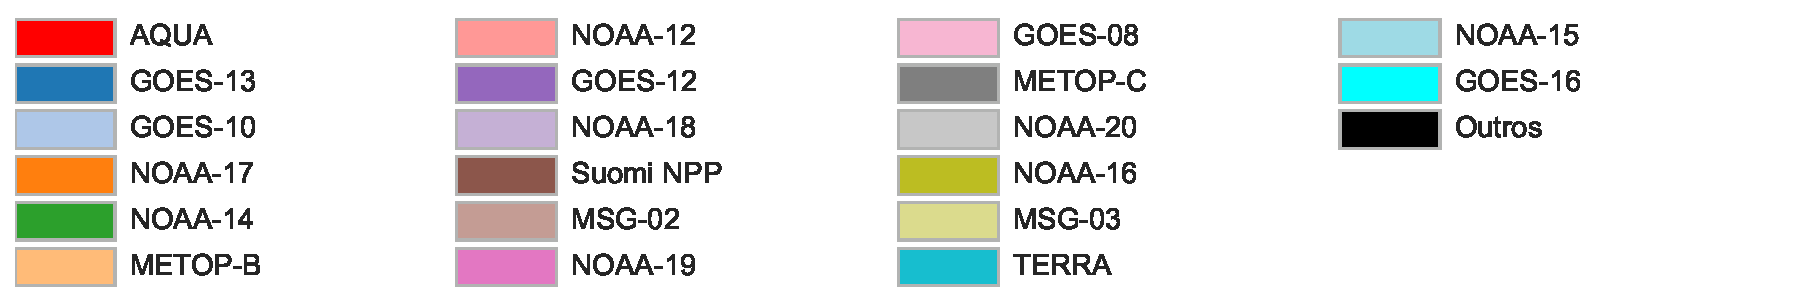
\includegraphics[width=35em]{cores_satelites}
    \end{center}
    \legend{Fonte: O Autor}
    \label{fig:cores_satelites}
\end{figure}


.... removido satélites ATSR .... removido satélites TRMM



....

A implementação das áreas dos focos, chamado de medições, usou os dados de satlélites de forma fixa no código (hardcoded). Apesar de exister bibliotecas especializadas em cálculos de órbitas de satélite, como a Orbital, essa abordagem foi escolhida a fim de evitar a necessidade de internet para execução do programa e simplificar o código. \par

Para simplificar e otimizar a implementação da parte das áreas dos focos, foi\par

------

A separação em quadrantes também foi planejada para melhorar o desempenho do processamento. Ao dividir o problema em partes menores, é possível resolver cada uma de forma paralela, pois as avaliações dos quadrantes são independentes entre si. Além disso, a separação em quadrantes otimiza ainda mais o processamento da junção espacial, que se beneficia quando os quadrantes para a interseção não são muito grandes. No entanto, é importante considerar que quanto maior o quadrante utilizado, menos avaliações são necessárias, mas a precisão da área queimada também é reduzida. Como se trata de um espaço bidimensional, a complexidade computacional da avaliação em relação à quantidade de quadrantes é $O(n^2)$. \par

\begin{figure}[H]
    \caption{Diferença da avaliação para diferentes tamanhos de quadrantes.}
    \begin{center}
        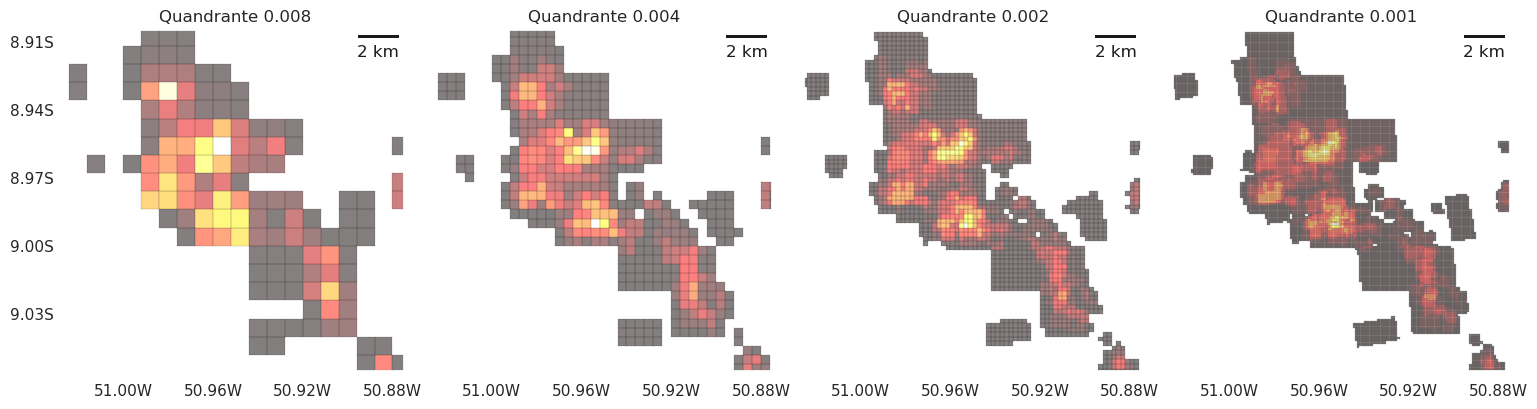
\includegraphics[width=35em]{diferenca_entre_quadrantes}
    \end{center}
    \legend{Fonte: O Autor}
    \label{fig:diferenca_entre_quadrantes}
\end{figure}

Com base em experimentos, foi constatado que o uso de quadrantes muito pequenos (com menos de 0,002 graus quadrados) não aumentam significativamente a precisão dos resultados e tornam a execução muito mais demorada.



%%%%%%%%%%%%%%%%%%%%%%%%%%%%%%%%%%%%%%%%%%%%%%%%%%%%%%%%%%%%%%%%%%%%%%%%%%%%%%%

\chapter{Resultados e Discussão}
\label{chp:resultados_discussão}

\section{Metodologia da avaliação}
\label{sec:metodologia_avaliacao}

Para a avaliação, usamos uma Tabela de Contingência modificada (ver Tabela \ref{table:matriz_de_confusao}) de forma que acomoda valores contínuos, representando o percentual de área queimada (\textit{soft classification}). Esse método de avaliação foi baseado em \citet{libonati2015algorithm}, que também aplicou a mesma técnica de avaliação para avaliar o produto AQ1km. A Tabela apresenta duas classes de interesse, ``Queimado'' e ``Não queimado'', de forma a comparar elas com um método de referência, nas colunas, e um método de interesse, nas linhas. A partir dessa comparação surgem os valores de Verdadeiro Positivo (TP), Falso Positivo (FP), Falso Negativo (FN) e Verdadeiro Negativo (TN).

\begin{table}[htbp]
\centering
\caption{Tabela de Contingência.}
\begin{tabular}{ccccc}
\toprule
 \multicolumn{2}{c}{} & \multicolumn{3}{c}{\textbf{Referência}} \\
 \cline{3-5}
 \noalign{\smallskip} % space
 \multicolumn{2}{c}{}                  & \textbf{Queimado} & \textbf{Não queimado} & \textbf{Total} \\
\midrule
 \multirow{3}{*}{\textbf{\shortstack{Método\\ proposto}}} & \textbf{Queimado}     & TP       & FP           & TP + FP \\
                        & \textbf{Não queimado} & FN       & TN           & FN + TN \\
                        & \textbf{Total}        & TP + FN  & FP + TN      & TP + FP + FN + TN \\
\bottomrule
\end{tabular}
\legend{Fonte: \citet{libonati2015algorithm}, modificado pelo autor}
\label{table:matriz_de_confusao}
\end{table}

A versão tradicional da Tabela de Contingência, também chamada de matriz de erro ou matriz de contingência, é comumente usada para avaliar problemas de classificação pesada (\textit{hard classification}), em que para cada objeto é atribuído uma classe única e sem classificações probabilísticas. No entanto, quando se trata de mapear a área queimada, a abordagem é um pouco mais complexa devido à natureza contínua e gradual da queima. Em vez de apenas classificar um quadrante como queimado ou não queimado, é necessário considerar a porcentagem da área efetivamente queimada dentro do quadrante. Essa abordagem é documentada em \citet{BINAGHI1999935} para a \textit{soft classification} utilizando a teoria dos conjuntos disjuntos.

Seja $p_r$ a avaliação de um quadrante pelo método de referência e $p_p$ a avaliação pelo método proposto, utilizamos as equações definidas em \ref{eqn:def_values} para calcular os valores TP, FP, FN e TN da Tabela de Contingência. Essas equações podem ser compreendidas usando a noção intuitiva de conjuntos, onde a operação $min$ representa a união e a subtração representa a diferença de dois conjuntos. Desse forma, a união de $p_r$ e $p_p$ indica o valor em que tanto o método proposto quanto o de referência concordam, resultando nos valores de TP. O mesmo pensamento vale também para o TN. Para os valores de erros, FN e FP, o resultado é extraído a partir de uma diferença que satura em zero. O valor de FP é zero quando $p_p \le p_r$, indicando que não há superestimação. Da mesma forma, o valor de FN é zero quando $p_r \le p_p$, indicando que não há subestimação.

\begin{equation} \label{eqn:def_values}
\begin{split}
	TP & = min\left(p_r, p_p\right) \\
	TN & = min\left(1 - p_r, 1 - p_p\right) \\
	FP & = max\left(p_p - p_r, 0\right) \\
	FN & = max\left(p_r - p_p, 0\right)
\end{split}
\end{equation}

Com esses dados, calculamos algumas métricas que nos ajudam a entender os resultados e melhor avaliar a solução proposta. A acurácia geral (OA), definido na Equação \ref{eqn:def_oa}, e o Índice de Sucesso Crítico (CSI), definido na Equação \ref{eqn:def_csi}, estão relacionadas. Enquanto a primeira leva em conta todos os dados de classificação, a segunda omite a informação dos verdadeiros negativos. Isso pode ser bom para o caso das queimadas, em que a classe ``Não queimado'' é muito mais frequente que a classe ``Queimado''. Para esses caso, pode-se entender que a métrica CSI foca na classificação correta da classe que seria ``difícil'' de acertar.

\begin{equation} \label{eqn:def_oa}
  OA = \frac{TP + TN}{TP + FP + FN + TN}
\end{equation}

\begin{equation} \label{eqn:def_csi}
  CSI = \frac{TP}{TP + FP + FN}
\end{equation}

Outras duas métricas importantes relacionadas são o Erro de Omissão (OE), definido na Equação \ref{eqn:def_oe}, e o Erro de Comissão (CE), definido na Equação \ref{eqn:def_ce}. O OE representa a proporção de elementos que deveriam ser classificados como queimados, mas foram erroneamente classificados como não queimados, ou seja, houve uma omissão. Por outro lado, o CE representa a proporção de elementos que foram classificados como queimados, mas que deveriam ser classificados com não queimados, em outras palavras, houve uma comissão. O valor dessas métricas fica entre 0 e 1 e quando menor, mais preciso é o modelo.

\begin{equation} \label{eqn:def_oe}
  OE = \frac{FN}{FN + TP}
\end{equation}

\begin{equation} \label{eqn:def_ce}
  CE = \frac{FP}{FP + TP}
\end{equation}

O Viés (B) é um indicativo de qual a tendência que o modelo seguiu. Um valor menor que 1 indica que o modelo está classificando menos áreas queimadas do que deveria. Caso o valor for maior que 1, está classificando mais áreas queimadas comparado a referência. Quando a métrica vale 1 a quantidade de áreas classificadas como queimada é a mesma. Essa métrica não deve ser usada como indicativo de precisão porque, mesmo quando vale 1, pode não haver correspondência com a classificação correta de áreas queimadas do modelo com as áreas queimadas da referência.

\begin{equation} \label{eqn:def_b}
  B = \frac{TP + FP}{TP + FN}
\end{equation}

O Coefiente de Dice (DC), também conhecido como Índice de Sørensen–Dice, é muito usado em processamento de imagens para calcular a similaridade de duas imagens, fazendo um sobreposição de seus valores. O valor fica entre 0 e 1, em que 1 representa uma sobreposição perfeita e valores próximos de 0 indicam uma maior taxa de erro. A equação de DC é similar a CSI, porém com um peso maior aplicado aos Verdadeiros positivos.

\begin{equation} \label{eqn:def_dc}
  DC = \frac{2 * TP}{2 * TP + FP + FN}
\end{equation}

\section{Aplicação da metodologia}

Nesta seção, é apresentado como o método de avaliação foi aplicado para comparar o método proposto de cálculo de áreas queimadas em relação ao estado da arte. Para isso, utilizamos o produto AQ30m como referência e comparamos, lado a lado, o método proposto, o produto MDC64A1 e o produto AQ1Km. Os dados do produto MDC64A1 foram obtidos a partir do site AppEEARS (\url{https://appeears.earthdatacloud.nasa.gov/}). Os dados do AQ30m podem ser visualizados e baixados de forma simples pelo site do Programa Queimadas (\url{https://queimadas.dgi.inpe.br/queimadas/aq30m}). Para obter os dados do AQ1Km foi necessário fazer uma solicitação para o INPE por e-mail, a resposta foi informando o servidor FTP para download dos produtos em formato Shapefile.

Os produtos têm resoluções diferentes, 30m, 500m e 1km respectivamente para AQ30m, MDC64A1 e AQ1km. Com isso, é necessário fazer uma transformação de forma que todos os produtos utilizados na avaliação estejam na mesma resolução. Há diferentes formas de fazer isso, em \citet{BOSCHETTI2004280} é apresentado um método que minimiza os erros de comissão e omissão do processo de transformar dados de área queimadas de resolução maiores em resoluções menores. 

Esse trabalho classificou os quadrantes de forma binária, em queimado e não queimado, o que altera o resultado do total de área queimada. Nesse sentido, a Figura \ref{fig:diferenca_resoluções} mostra a diferença do total da área queimada entre a versão original, de resolução 30m, e três variações de limiares em uma resolução maior. Os valores de cada quadrante foram obtivos fazendo uma intercção entre os limites do quadrante e o polígono original, depois disso é filtrado apenas os quadrantes que apresentaram um valor acima do limiar testado. Ou seja, todos os quadrantes maiores que 0, 0.5 ou igual a 1 são apresentados, respectivamente, na segunda, terceira e quarta imagem.

\begin{figure}[H]
    \caption{Redução da resolução do produto AQ30m (a esquerda) para uma resolução de aproximadamente 330m usando diferentes limiares. A segunda imagem contém todos os quadrantes com valores maiores que 0. A terceira imagem mostra quadrantes que tem pelo menos metade de sua área coberta. A última imagem mostra apenas quadrantes totalmente cobertos pelo polígono original.}
    \begin{center}
        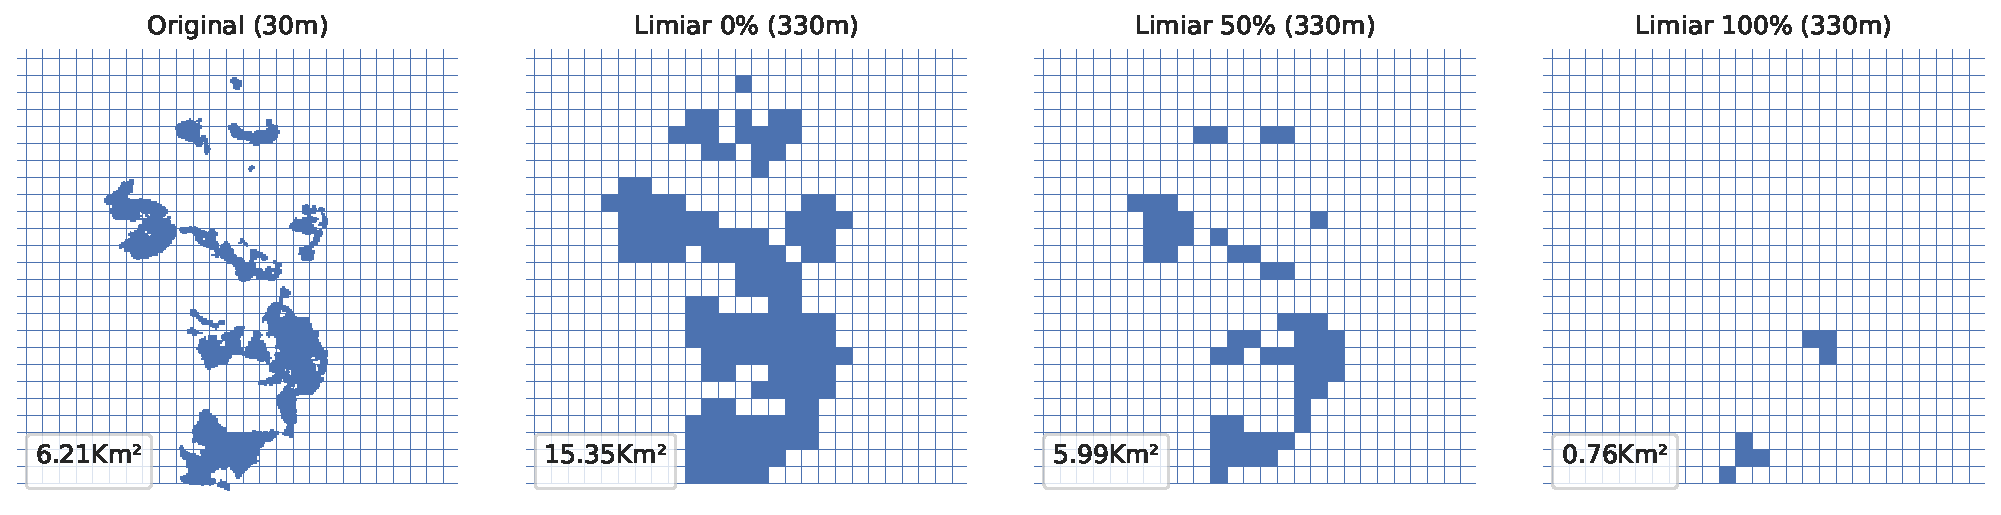
\includegraphics[width=35em]{diferenca_resoluções}
    \end{center}
    \legend{Fonte: O Autor}
    \label{fig:diferenca_resoluções}
\end{figure}

Uma outra forma de transformar uma resolução maior para uma menor é manter o valor contínuo resultante da intersecção das extremidades do quadrante com o polígono original. Com isso, o problema dos erros de comissão e omissão da abordagem anterior não estão presentes nessa abordagem, como mostrado na imagem \ref{fig:resolução_continua}. A área queimada praticamente não foi alterada entre as duas imagens. A diferença foi cerca de 40m a menos em relação a imagem original, que pode ser devido ao método usado para cálculo de área espacial a partir do polígo ou problemas de arredondamento de ponto flutuante.

\begin{figure}[H]
    \caption{Redução da resolução do produto AQ30m (a esquerda) para uma resolução de aproximadamente 330m sem perda significativa de área queimada. Cada quadrante na imagem da direita representa a porcentagem do quadrante que está classificado como queimado.}
    \begin{center}
        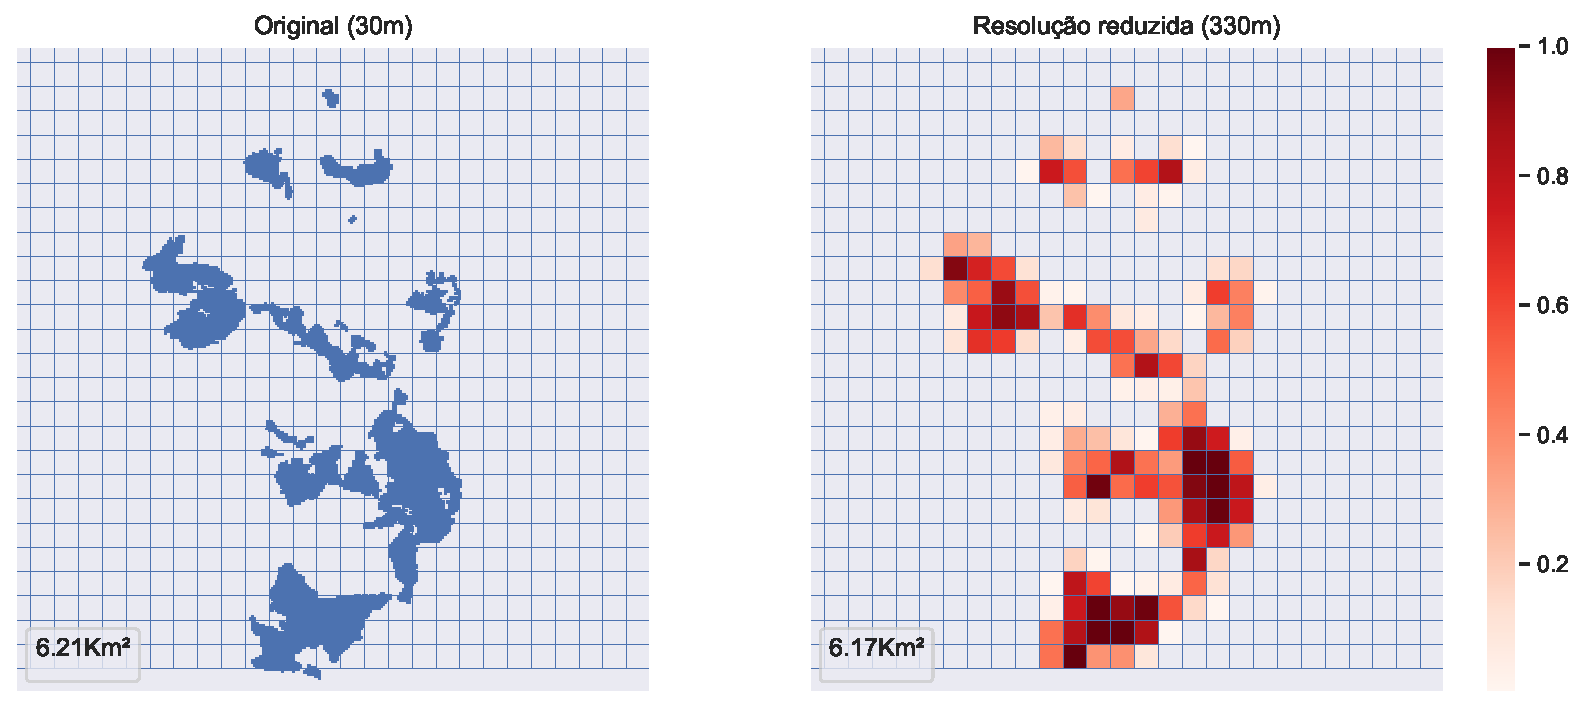
\includegraphics[width=25em]{resolução_continua}
    \end{center}
    \legend{Fonte: O Autor}
    \label{fig:resolução_continua}
\end{figure}

Além do obstáculo das resoluções diferentes entre os produtos, um outro problema é a escolha da porção territorial a ser avaliada. Para simplificar e possibilitar a comparação entre diversos trabalhos mencionados (como em \citet{libonati2015algorithm}), foi escolhido usar as áreas delimitadas pelo WRS-2, descritas na Figura \ref{fig:orbitas_ponto_landsat}. O produto AQ30m também é distribuído seguindo o mesmo sistema, mas com uma diferença que demanda atenção. No sistema WRS-2, as órbitas-ponto podem ter intersecção com outras órbitas-ponto vizinhas. Caso isso fosse mantido no produto AQ30m, poderia haver contagens repetidas de uma mesma área queimada nas extremidades da área delimitada pela órbita-ponto. Para solucionar esse problema, foi usado uma versão modificada da grade WRS-2, obtida a partir de \url{http://www.dgi.inpe.br/documentacao/grades}, que é um mosaico sem sobreposiç˜ão.

\section{Resultados apresentados}


O método em sí é geral para qualquer entrada de focos de satélites, e retorna no final polígonos representando áreas geográficas associadas a um valor que indica a área queimada dentro desse polígono. Variando a entrada do método e o agrupamento dos resultados preliminares, pode-se obter diferentes resultados finais. \par


%%%%%%%%%%%%%%%%%%%%%%%%%%%%%%%%%%%%%%%%%%%%%%%%%%%%%%%%%%%%%%%%%%%%%%%%%%%%%%%

\chapter{Considerações Finais}

%%%%%%%%%%%%%%%%%%%%%%%%%%%%%%%%%%%%%%%%%%%%%%%%%%%%%%%%%%%%%%%%%%%%%%%%%%%%%%%


\bibliographystyle{abntex2-alf}
\bibliography{biblio}

\end{document}
